% !TEX encoding = UTF-8 Unicode
\documentclass[submitted]{article}
\usepackage{i}
\usepackage{els}
\usepackage{lib}
\usepackage{mat2}
\usepackage{geoA4}
\usepackage{mdframed}
\usepackage{notate}
\usepackage{aut}
\usepackage{standalone}
\usepackage{caption}
\captionsetup{font=footnotesize}

\setlength{\parskip}{0em}
\renewcommand{\diff}{d}
\renewcommand{\Mink}{Minkowski\xspace}
\newcommand{\texts}[1]{\text{\footnotesize{#1}}}
\newcommand{\stth}[1]{}
\newcommand{\stt}[1]{}
\newcommand{\faradaymn}{\ensuremath{f\mn}}
\newcommand{\faraday}{\ensuremath{f}}
\newcommand{\christoffelmnt}{\christoffel{\mu}{\nu}{\tau}}

\newcommand{\labtag}[1]{\label{#1}}
\newcommand{\labtagtwo}[1]{\label{#1}}
\newcommand{\mpage}[1]{}
\newcommand{\wpo}{worldpoint\xspace}
\newcommand{\ctmr}{charge-to-mass ratio\xspace}
\newcommand{\ctmrf}{\ensuremath{\hfrac{e}{m}}\xspace}
\newcommand{\xadx}{$\xn$ and $\xn$ + $d\xn$\xspace}
\newcommand{\xpdx}{$\xn+d\xn$}
\newcommand{\ctmrg}{\ensuremath{\hfrac{m_g}{m}}\xspace}
\newcommand{\ctmrd}{\ensuremath{\hfrac{\rho}{\mu}}\xspace}
\newcommand{\RTo}{\ensuremath{\varphi\tmn=-k f^\tau_\nu u_\mu}\xspace}
\newcommand{\RTt}{\ensuremath{\varphi\tmn=-f^\tau_\nu u_\mu}\xspace}
\newcommand{\FT}{\ensuremath{\varphi\tmn = - g_{\mu \nu} h^{\rho \sigma} \hfrac{\partial \Phi}{\partial x_\sigma}}\xspace}
\newcommand{\Gtmnbar}{\ensuremath{\bar{\Gamma}\tmn}\xspace}
\newcommand{\til}{timelike\xspace}
\newcommand{\spl}{spacelike\xspace}
\renewcommand{\oe}{;~o.e.{}}
\renewcommand{\me}{;~m.e.{}}
\newcommand{\oemph}[1]{\emph{#1}}
\newcommand{\memph}[1]{\emph{#1}}
\crefalias{pippo}{enumi}
\crefformat{enumi}{#2#1#3}


\newcommand{\PRZL}{\citetitle{Reichenbach1928}\xspace}
\newcommand{\Reich}{Reichenbach\xspace}



\renewcommand{\rzlp}[2]{(\cite[#1]{Reichenbach1928}; tr.\ #2)\xspace}
\renewcommand{\rzlap}[2]{(\cite[#1]{Reichenbach1928}; tr.\ [#2])\xspace}


\makeatletter
\def\tagform@#1{\maketag@@@{[\ignorespaces#1\unskip\@@italiccorr]}}
\makeatother

\creflabelformat{equation}{#2[\textup{#1}]#3}

%\titleformat{\section}
%{\normalfont\bfseries}{\rom{\thepart}.\thesection}{1em}{\normalsize\bfseries\boldmath{#1}}


\newmdenv[linecolor=black]{infobox}

\title{\scare{Geometrization of Physics} vs.\ \scare{Physicalization of Geometry}. The Untranslated \Ap to Reichenbach's \PRZL}

\begin{document}
\maketitle


\begin{abstract}
This article provides an overview of the \Ap to Reichenbach's 1928 \PRZL, which was not included in the widely read English translation of the book published 30 years later. The \Ap, after a lengthy introduction of the basic concepts of differential geometry and of the problem of the their physical interpretation, presents an intentionally artificial example of geometrization of the electromagnetic field, by allowing \st to have torsion, in addition to curvature. At that time, it was a widespread opinion that, after Einstein's \scare{geometrization} of the gravitational field, the \scare{geometrization} program should be extended to the other known field. However, Reichenbach aimed to prove that dressing a physical field in a geometrical \scare{cloak} is a display of mathematical sophistication, not of physical insight. A geometrical \scare{cloak}, as Reichenbach put it, is useful only if it reveals something new about the shape of the \scare{body} under it, the physical field. The present study, through comparison of Newtonian gravitation (Newton-Cartan theory) with Friedrichs's geometrization, indicates that Reichenbach's geometrization attempt was doomed to failure. Nevertheless, it is argued, the philosophical message of the \Ap should be considered an integral part of the line of argument of \PRZL, particular its last chapter on \gr. The book's main message was that \gr was not the beginning of the new era of \scare{geometrization of physics}, but the culmination of a historical process of \scare{physicalization of geometry}.
\end{abstract}



\begin{keywords}
Reichenbach, Hans \sep General Relativity \sep Unified field theory \sep Geometrization 
\sep Newton-Cartan Theory
\end{keywords}

%TODO FORMULAS
%TODO cop

\section*{Introduction}

For today's readers of Hans Reichenbach's \citetitle{Reichenbach1958} \citep{Reichenbach1958}, it might come as a surprise that the book is missing the translation of an \Ap entitled \scare{Weyl's Extension of Riemann's Concept of Space and the Geometrical Interpretation of Electromagnetism}. A reference to a no-longer-existing \S46 on page ~17 is the only clue of its existence. The \Ap covered some 50 pages of the German original, the \PRZL \citep{Reichenbach1928}-not few considering that Reichenbach dedicated only half a score pages more to \gr. The editors of the English translation, Maria Reichenbach and John Freund, had prepared a typescript of the translation of the \Ap \citep[041-2101]{HR} including the transcription of the mathematical apparatus, which was considerably heavier than that in the rest of the book \footnote{Henceforth, the English translations of \PRZL are taken from \cite{Reichenbach1958}; translations of the \Ap are taken from \cite[041-2101]{HR}. In the latter case, page numbers are enclosed in square brackets}. However, they must have decided not to include it into the published version eventually. By the end of the 1950s, Weyl's geometrical interpretation of electromagnetism was at most of antiquarian interest. The mathematical effort the readers were asked to familiarize with the subject might have appeared not worth the modest philosophical gain. With the important exception of a pathbreaking paper by Alberto \citet{Coffa1979}, the case of the missing \Ap did not seem to have attracted attention in the theoretical and historical literature since then \ascitep{Giovanelli2016}.

The context in which the \Ap was written is briefly recounted by Reichenbach himself in an unpublished autobiographical sketch \citep[044-06-25]{HR}. Reichenbach started to work on the \PRZL in March 1925. The drafting of the manuscript was interrupted several times, but some of its core parts were finished at the turn of 1926, when Reichenbach was negotiating a chair for the philosophy of physics in Berlin \citep{Hecht1982}. \qt{In March-April 1926, Weyl's theory was dealt with, and the peculiar solution of \S49 was found. At that time, the entire \Ap was written. (correspondence with Einstein). Talk at the physics conference in Stuttgart}{March-April 1926 wurde die "Weylsche Theorie bearbeitet u. die eigentümliche LÃsung des \S49 gefunden. Auch wurde damals der ganze Anhang geschrieben. (Korrespondenz mit Einstein) Vortrag auf d. Physikertag in Stuttgart} \citep[044-06-25]{HR}. This short reconstruction is confirmed by independent textual evidence \ascitep{Giovanelli2016}. In March 1926, after making some critical remarks on Einstein's newly published metric-affine theory \citep{Einstein1925a}, Reichenbach sent Einstein a 10-page \scare{note} that would turn out to be an early draft of \S49 of the \Ap. The typescript of the note is still extant \citep[025-05-10]{HR}. Einstein's objections and Reichenbach's replies reveal that contrary to \citets{Coffa1979} claim, Reichenbach's defense of geometrical conventionalism against Weyl's geometrical realism \scitep{Ryckman1995} was not the motivation behind Reichenbach's note.

Reichenbach was concerned with the more general problem of the meaning of a \scare{geometrization} of a physical field. At that time, it was a widespread opinion that after general relativity had successfully geometrized the gravitational field, the next obvious step was to \scare{geometrize} the electromagnetic field \segcitep{Weyl1918a,Eddington1921,Weyl1921e}. However, according to Reichenbach, this research program-the so called \uftp \scitep{Vizgin1994,Sauer2014,Goenner2004}-was based on a fundamental misunderstanding of the nature of Einstein's geometrical interpretation of the gravitational field. To prove his point, Reichenbach put forward his own attempt of a geometrical interpretation of the electromagnetic field. Thus, he hoped to demonstrate that such geometrization was not much more than a mathematical trickery that in itself does not constitute a gain in physical knowledge. Einstein, in spite of having found some significant technical mistakes in Reichenbach's theory, agreed, at least superficially, with Reichenbach's \scare{philosophical} message \citep{Lehmkuhl2014}. Against Einstein's advice, Reichenbach presented this material in public at the Stuttgart meeting of the German Physical Society \citep{Reichenbach1926d}. Later, he included it in the manuscript of the book he was working on as part of a longer \Ap. After some struggle in finding a publisher, the manuscript of the \PRZL was finished in October 1927 and published the following year by De Gruyter \citep[044-06-25]{HR}.

The correspondence between Reichenbach and Einstein has been already discussed elsewhere \acitep{Giovanelli2016}. In the present article, I aim to offer an introduction to the \Ap itself. Besides the note that Reichenbach sent to Einstein, which became \S49, the \Ap entails over 40 pages of additional material, that are worth further investigation. As the present paper will try to demonstrate, the philosophical message of the \Ap should be considered an integral part of the line of argument of \PRZL and, in particular, of its last chapter dedicated to \gr. As Reicenbach pointed out, according to \gr, the universal effect of gravitation on all kinds of measuring instruments defines a \emph{single geometry}, a, in general, non-flat Riemannian geometry. \q{In this respect, we may say that gravitation is \oemph{geometrized}} \rzlp{294\oe}{256}. We do not speak of deformation of our measuring instruments \q{produced by the gravitational field}, but we regard \q{the measuring instruments as \scare{free from deforming forces} in spite of the gravitational effects} \rzlp{294}{256}. However, such a \emph{geometrical explanation} is, according to Reichenbach, not an explanation at all, but merely a codification of a matter of fact. Reichenbach insisted that, also in \gr, it was still necessary to provide a \emph{dynamical explanation} of the observed behavior of \rac, although a dynamical explanation of a new kind. Even if \q{we do not introduce a force to explain the \emph{deviation} of a measuring instrument from some normal geometry}, we must still invoke a force as a \emph{cause} for the fact that \q{\oemph{there is a general correspondence \origins{einheitliches Zusammenstimmen} of all measuring instruments}} \rzlp{294\oe}{256}, that all agree on a non-flat Riemannian geometry depending on the matter distribution. 

Indeed, according to Einstein's theory, \gr teaches us that we may consider the \q{effect of gravitational fields on measuring instruments to be of the same type as all known effects of forces} \rzlp{294}{257}. What is characteristic of gravitation respect to other fields is the \emph{universal coupling} of gravitation and matter. Measuring instruments made of whatever fields and particles can be used to explore the gravitational field, and the result of such measurements is independent of the device. As a consequence, it becomes impossible to separate the measuring instruments that measure the background geometry (\rac, light rays, uncharged test particles) from those that measure the dynamical field (charged test particles). The geometrical measuring instruments have become indicators of the gravitational field. However, this does not imply that it is \q{\oemph{the theory of gravitation that becomes geometry}}; on the contrary, it implies that \q{\oemph{it is geometry that becomes an expression of the gravitational field}} \rzlp{294\oe}{256}. For the reader of the English translation, Reichenbach's line of argument makes a short appearance at the end of the sections dedicated to \gr and is then interrupted abruptly. However, in the original German, Reichenbach's line of argument, it is picked up again and developed for further 50 pages in the \Ap. Thus, the latter is nothing but the second half of an argumentative arch whose first half had been erected in the last chapter of the book. 

This study demonstrates how in the \Ap, starting from the affine connection instead of that from the metric, Reichenbach formulated a theory that seems to \scare{geometrize} both the gravitational and the electromagnetic fields. However, unlike general relativity, Reichenbach's theory does not add any new physical knowledge that was not already entailed in previous theories. Thus, the geometrization of a field is not in itself a physical achievement. A comparison with a geometrization of Newtonian gravity suggested by Kurt \citet{Friedrichs1928} at around the same time, provides the simple reason why Reichenbach's attempt was bound to fail\footnote{This geometrization is known as Newton-Cartan theory, since it was developed independently by \cite{Cartan1923,Cartan1924}; \scite{Malament2012}}. Nevertheless, Reichenbach's theory is revealing of the philosophical message that \PRZL was meant to convey. Undoubtedly, general relativity has dressed the distinctive feature of gravitation (its universal coupling with all other physical entities) in a shiny geometrical \scare{cloak} (a Riemannian geometry with variable curvature). However, in Reichenbach's preferred analogy, one should not mistake \qt{the cloak \origins{Gewand} for the body that it covers}{Man darf nicht das Gewand für den KÃrper halten, der darunter steckt} \rzlap{354}{493}. Contrary to widespread belief, \gr was not the dawn of the new era of \scare{geometrization of physics} that was supposed to dominate 20th-century research for a \uft; \gr was the culmination of a historical process of \scare{physicalization of geometry} that had begun in the 19th century.

\section{The Appendix to the \PRZL. Overview and Structure}
\label{overview}

\Gr rests formally on Riemannian geometry. The latter is based on the \scare{hypothesis} that the squared distance $ds$ between two neighboring points; \xadx is a homogeneous, second-order function of the four coordinate differentials. In Einstein's notation (where summation over repeated indices is implied), it reads as follows:

\begin{equation}\label{eq:lineelement}
ds^2=\gmn dx_\mu dx_\nu\.
\end{equation}
%
As is well-known, the coefficients $\gmn=g_{\nu\mu}$ are at the same time (a) the components of the metric (\scare{measurement}) field---a set of 10 numbers that serve to convert coordinate distances $dx_\nu$ between two closed by \st points into real distances $ds=\pm 1$--- and (b) components of the gravitational field. The numerical value of the $ds$ has a physical meaning, if it can be considered as the result of a measurements, which inevitably demand a unit in which to measure. In \rt, \rac are at rest relative, perform orthogonal measurements, clocks supply $d s=-1$, and rods $d s=+1$. \q{Why are these measuring instruments adequate for this purpose?} \rzlap{331}{463}. The fundamental property that makes them suitable for measuring the $ds$ was outlined by Reichenbach in \S4 of the \PRZL \rzlp{26--27}{17}. One can chose, say, $n$ spacings between the atoms of a rock-salt crystal as a unit of length $ds=1$. As it turns out, two identical crystals that have the same length when lying next to each other are always found to be equally long after having been transported along different paths to a distant place. The same holds for unit clocks. One can arbitrarily choose $n_1$ wave crests of cadmium atom emitting the red line or $n_2$ of a sodium atom emitting the yellow line as a unit of time $ds=-1$. However, the ratio $n_1/n_2$ happens to be a natural constant.


\Gr, as a testable theory, stands or falls with this empirical fact \ascitep{Giovanelli2014}. However, it would be possible to think of a world in which \rac does not have this peculiar \scare{Riemannian} behavior. In this world, it would still be possible to formulate a definition of congruence, that is, a definition of the equality of $ds$'s. However, such definition would not be unique. The units of length would have to be given for every space point, and we could not simply rely on Paris standard meter. In a Riemannian world, if we know the length of a room, we also know the number of unit rods that we can place along one of its walls \rzlap{333}{464}. In a non-Riemannian world, such number would depend upon the path by which the rods were actually brought into the room \rzlap{333}{464}. \q{Such conditions may seem very strange, but they are certainly possible, and if they were real, we would surely have adapted ourselves to them} \rzlap{333}{464}. Obviously, setting randomly different units of measure at every point would be of little use for the people in such a world. Instead, they would search for a \q{geometrical method which would characterize the law of \emph{change in length} during transport; that is, they would search for \scare{the law of displacement} \origins{Verschiebungsgesetz}} \rzlap{333}{464}: how much lengths change when transported at infinitely close points.

%The length of $l^2=\gmn A^\mu A^\nu$ allows one to calculate the length of vectors from their components up to a constant. 



Thus, the geometrical problem of formulating such a \scare{law of displacement} arises. According to Reichenbach, this problem was addressed and solved by \citet{Weyl1918a,Weyl1918b}. Weyl's \q{solution certainly constitutes a mathematical achievement of extraordinary significance regardless of its physical applicability} \rzlap{333}{464}. One can think of $d\xn$ as the components of a vector $A^\tau$. Weyl realized that there are two separate operations of comparison of vectors $A^\tau$. Using a somewhat idiosyncratic language, Reichenbach calls the \emph{metric} the operation of \emph{distant-geometrical} comparison of lengths of vectors. At every point, once we know the numerical values of the components of a vector $A^\mu$ in a certain coordinate system, the metric \gmn allows one to calculate its length, a single number $l^2=\gmn A^\mu A^\nu$. If a different unit of measure is chosen (inches instead of cm), then one would obtain a different number $l'=\lambda l$. However, the ratio $\lambda$ is regarded as an absolute constant \citep[see][102]{Weyl1919a}. Weyl realized that, on the contrary, in the general case, it is not possible to establish whether two vectors $A^\tau$ and $A'^\tau$ at different places have the same direction by simply inspecting their components. Reichenbach typically calls \emph{displacement} the operation of \emph{near-geometrical} comparison of the direction of vectors that takes into account the intermediary steps needed to \scare{displace} or transfer a vector from one place to another. In Reichenbach's characterization, Weyl discovered a type of space more general than the Riemannian space, in which the near-geometrical operation of displacement, rather than the distant-geometrical metrical comparison, represents the most fundamental operation. 
 
%If a vector, if one someone Earch 3 cm and 6 cm, we now that two, since they agree on the same unit, cm. The change unit, 7,62 and 15,25. One vector is still two times larger than the other; this can be established once and further.

%If a vector, 3 and 6, in earth, we now that two, it would also might be in another place, an find ie one of the other, since would depend on the path of transport

In particular, Weyl envisaged a geometrical setting \q{[t]he comparison of lengths by means of a metric is \textelph{now} replaced by a comparison of lengths through displacement} \rzla{336}{469}. The ratio of units is allowed to change from point to point, thus $l'=\lambda(\xn)l$ is an arbitrary function of the coordinates. Weyl found that in such a geometry, the change of length $l$ of a vector transported to a nearby point is expressed by the formula $d (\log l)=\kappa_\sigma dx_\sigma$, where $\kappa_\sigma$ is a vector field. The mathematical \scare{discovery} of the independence of the operation of displacement and of the metric had important implications in \st physics. On the one hand, it turns out to be advantageous to present \gr as theory based not solely on the metric \cref{eq:lineelement} but also on two separate geometrical structures and to impose as a compatibility condition that the length of equal parallel vectors is the same. On the other hand, by weakening such a compatibility condition, one can open new mathematical degrees of freedom that can be used to incorporate the electromagnetic field into the geometry of \st. In particular, \citet{Weyl1918a} identified $k_\sigma$ with the electromagnetic four-potential \segcitep{Scholz1994}. Other strategies of \scare{geometrizing} the electromagnetic field were evaluated when Reichenbach was writing the \Ap. One can keep Riemannian geometry but increase the number of dimensions \segcitep{Einstein1927a,Einstein1927b} or abandon the restriction that $ds$ is a quadratic form \citep{Reichenbaecher1925}. However, Reichenbach did not consider these theories and only discussed Weyl's \german{Ansatz} and its further developments.

\begin{inparaenum}[(1)] The goal of the \Ap to the \PRZL was to outline \item a generalization of Weyl's mathematical approach based on the work of \citet{Eddington1923} and \citet{Schouten1922}. In particular, Reichenbach's terminology and notation is taken from the German translation \citep{Eddington1925a} of Eddington's textbook on relativity \citep{Eddington1923}. However, Reichenbach followed \citet{Schouten1922} in adopting a more general definition of the operation of displacement. This mathematical treatment, in Reichenbach's parlance, amounts to provide \item a \emph{conceptual definition} of the operation of displacement, without asking about its physical realization or interpretation. The second step \item was to investigate the physical applicability of such a mathematical apparatus. This means dealing with the empirical question whether or not there are objects in nature that behave according to the operation of displacement. This second step amounts to provision of a \emph{coordinative definition} of the operation of displacement. After a coordinative definition has been chosen, Reichenbach \item presented an example of \emph{physical application} of such a mathematical apparatus. Reichenbach demonstrated that, by resorting to a sufficiently general definition of the operation of displacement with an appropriate physical interpretation, one could provide a geometrical interpretation of the electromagnetic field that was \scare{just as good} as the geometrical interpretation of the gravitational field provided by Einstein. \item Finally, Reichenbach reflected on the \emph{philosophical consequences} of his theory. By demonstrating that his geometrization of the electromagnetic field, although impeccable as geometrical interpretation, did not lead to any new physical results, Reichenbach concluded that geometrization in itself was not the reason why \gr was a successful physical theory. Thus, after a brief introduction of \S46, the \Ap is roughly structured in this way: \end{inparaenum}

\begin{enumerate}
 \item The conceptual definition of the operation of displacement (\S47)\todo{checl}
 \item The coordinative definition of the operation of displacement (\S 48)
 \item An example of a physical application of this mathematical apparatus (\S 49)
 \item The philosophical consequences (\S50)
\end{enumerate}


\section{The Conceptual Definition of the Operation of Displacement}

\subsection{Displacement Space and Metrical Space}

Let us assume that a coordinate system is spread over an \st region, so that each point is identified by a set of four numbers $x_\nu$ (where $\nu=1, 2, 3, 4$). This coordinatization is of course completely arbitrary. A vector $A^\tau$ placed at some point $P$ with coordinates \xn can be thought as an arrow or as the sum of its components $A^\mu$, the four numbers ($A_1$, $A_2$, $A_3$, $A_4$) that we associate with some point $P$. Given a vector with components $A^{\mu}$ in the coordinate $\xn$, the component $A^{\prime \mu}$ of the vector in the coordinates \xnpr is $A'^{\mu}=\left(\partial x^{\prime \mu} / \partial x^{\rho}\right) A^{\mu}$. A collection of four numbers $A^\mu$ that change according to this rule is defined as the contravariant components of a vector $A^\tau$. For example, the displacement vector, $d_\nu$ (the separation between two neighboring points), leading from $\xn$ to $\xn + d\xn$ is the prototype of a contravariant vector. In Euclidean geometry, it is always possible to introduce a Cartesian coordinate system in which two vectors are equal and parallel when they have the same components:

\begin{equation}\label{eq:samness}
A'^\tau-A^\tau=0\.
\end{equation}
%
One can move $A^\tau$ at $P$ with coordinates \xn to a neighboring point $P'$ with the coordinates $\xn+dx_\nu$ from $P$ and place a vector, $A'^{\tau}$, there. $dx_\nu$ might be called a \scare{displacement}\footnoteh{Transfer}. If the vector does not change its components, then it is the \scare{same} vector at a different point $P'$. 


However, this simple relation does not hold if we introduce curvilinear coordinates, \eg polar coordinates. The components of the vector change according to $A^{\mu}=\left(\partial x^{\prime \mu} / \partial x^{\rho}\right) A^{\rho}$. Since the partial derivatives vary from point to point, we cannot compare two vectors, even not at neighboring points. Two vectors might have different components because they are not equal and parallel or because the components have changed in a different way at different points\footnoteh{\Eg consider two unit vectors pointing on a plain along the $x$ direction: one at the point $(1,0)$ and another at the point $0,1$ in Cartesian coordinates. These two vectors have the same components $(1,1)$, that they are equal and parallel. In polar coordinates $\varphi,\vartheta$, however, the first has only a $\varphi$ component, whereas the second has only a $\vartheta$ component. Nevertheless, they are equal and parallel}. Thus, if one moves the vector to a neighboring point $dx_\nu$, one does not know whether the vector has remained the \scare{same} by simply looking at its components. In other words, we have lost the \scare{connection} (\german{Zusammenhang}) from a point to another. Since the affine geometry is the study of parallel lines, \citet{Weyl1918a,Weyl1918b} used to speak of the necessity of establishing a \scare{affine connection} (\german{affiner Zusammenhang}). However, it is relation of \scare{sameness} rather than parallelism that is relevant in this context. According to a nomenclature that was also widespread at that time, Reichenbach typically referred to the operation of \scare{displacement} (\german{Verschiebung}) as the small coordinate difference $d\xn$ along which the vector is transferred. Since the \scare{displacement} also indicates the vector $d\xn$, the expression \scare{transfer} (\german{\"Ubertragung}) was preferred by other authors \segcitep{Schouten1922,Schouten1923}.

\paragraph{Displacement}
%
To reinstate the \scare{connexion}, one needs to establish a rule to compare vectors at infinitesimally separated points. 

\begin{equation*}
dA^\tau = A^{\prime\tau}-A^{\tau}\.
\end{equation*}
%
Given a vector $A^\tau$ at \xn in any coordinate system, we need to determine the components vector $A'^\tau$ at $\xn+d\xn$ that is to be considered the \scare{same vector} as the given vector $A^\tau$, that is, $dA^\tau=0$. We expect that the vector at $\xn+\diff \xnpr$ will depend linearly on the vector at \xn; further, the change in the components between the two points will be proportional to the coordinate shifts $\diff \xn$. Thus, we expect a rule that takes the form:

\begin{equation}\label{eq:affine}
dA^\tau = \Gamma^\tau_{\mu\nu}A^{\mu} dx_\nu\.
\end{equation}
%
The quantity $\Gamma^\tau_{\mu\nu}$ has three indices, that is, entails $\tau$ possible combinations of $\mu \times \nu$ coefficients, which can vary arbitrarily from \wpo to \wpo. In other words, they are arbitrary continuous functions of the \xn. Notice that Reichenbach, following \citet{Schouten1922a}, did not impose the symmetry of the $\mu,\nu$, so that in general $\Gtmn \neq \Gtnm$. Thus, in four-dimensions, one has $4 \times 16 = 64$ coefficients, which reduce to $4 \times 10 = 40$, if $\Gtmn = \Gtnm$.

Starting with a vector $A^\tau$ at a point $P$ with coordinates \xn, one may displace this vector along $dx_\nu$ to the \wpo $P'$ with coordinates $\xn+dx_\nu$; using \cref{eq:affine}, one can compute the components vector $A'^\tau$ at $P'$ that is equal and parallel to $A^\tau$ at $P$ in any coordinate system. The \Gtmn is not a tensor. $\Gtmn=0$ in a Cartesian coordinate system, so that the components of a vector do not change under parallel transport. However, $\Gtmn\neq0$ in a different coordinate system, so that the components of a vector do change under parallel transport. Continuing this process step after step from $A'^\tau$ to $A''^\tau$, to $A'''^\tau$ and so on, we obtain a broken-line curve. As the size of each displacement goes to zero, this broken line becomes a continuous curve $x_\nu(s)$: 

\begin{equation}\label{eq:parallelgeodesics}
\frac{d {A}^{\mu}}{\dap} = \Gamma^\tau_{\mu\nu}A^{\mu} dx_\nu\,. 
\end{equation}
%
Let $P$ and $Q$ be two \wpo{}s connected by a curve. If a vector is given at $P$, then this vector may be moved parallel to itself along the curve from $P$ to $Q$; for given initial values of $A^\tau$, \cref{eq:parallelgeodesics} gives the unknown components of the vector $A'^\tau$, which is being subjected to a continuous parallel displacement, in which step is labeled by the parameter $\ap$. Thus, \cref{eq:parallelgeodesics} picks up the \emph{straightest among all possible curves} between $P$ and $Q$; that is, the lines whose direction along itself is parallel transported. At this stage, neither the notion distance nor angles between vectors have been defined. Nevertheless, the operation of displacement is sufficient to compare the length of parallel vectors, that is the length relative to other lengths along the \emph{same} straightest line. We can compare the lengths of any two sections of this curve, that is, determine the ratio of the \scare{number of steps} $\ap$ (the so-called affine parameter) involved in each of them.

\begin{wrapfigure}{L}{0.5\textwidth}
\centering
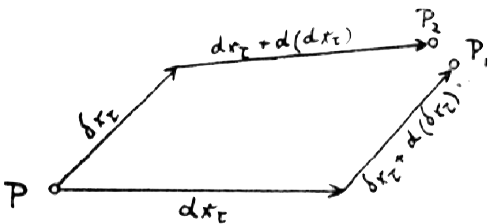
\includegraphics[scale=0.3]{reichenbachparallelogram.png}
\caption{\label{fig:reichenbachparallelogram} The nonexistence of infinitesimal parallelograms \citep[348]{Reichenbach1928}}
\end{wrapfigure}
%
The displacement is not assumed to be symmetric \asym. This implies that, \cop{if four neighboring infinitesimal vectors are parallel in pairs and equally long in the sense of the displacement, they will not form a quadrilateral. Thus, by transporting a vector parallel to itself starting from $P$, one will not arrive at the same point $P$. In the general displacement space, there are no infinitesimal parallelograms} $(d x)^{\mu}+(\delta x)^{\mu}-\Gamma_{\nu \alpha}^{\mu}(\delta x)^{\alpha}(d x)^{\nu}$\footnote{The difference between a symmetric connection and a non-symmetric one $\Gtmn-\Gamma^\tau_{\nu\mu}$ is a tensor of third rank $J_{\mu\nu,\tau}=\frac{1}{2} \Gtmn-\Gamma^\tau_{\nu\mu}=0$. This tensor is called an asymmetry tensor or torsion. However, Reichenbach did not introduce this notation (see below \cref{appendix}}). If we require the connection to be symmetric, the vectors will form a quadrilateral, and we will arrive at the same point $P$ \rzlap{348--349}{485--486}. However, the vector thus obtained will not be, in general, the same vector as the one we have started from; that is, it will not be equal and parallel to it. The parallel transport of a vector $A^\tau$ from $A$ to $B$ and from $B$ to $A$ is reversible (on transferring back along the same curve, you get back the initial vector at $P$); however, in general, parallel transport along a curve depends on the curve, not only on the initial and final points. Thus, the components of $A'^\tau$ at $B$ depend on the path chosen:

\begin{equation*}
A'^{\tau}-A^{\tau}=\int_{s} \Gtmn A^{\mu} d x_{\nu}\,
\end{equation*}
%
where the integral $s$ depends on the path. Given a vector at one point $P$, using the \Gtmn, one can determine which is the \scare{same} vector at the neighboring point $P'$. To determine which is the \scare{same} vector at a point $Q$ that is a finite distance from $P$, then we will have to \scare{transport} the initial vector along a succession of infinitesimal steps to reach the final point $Q$. However, the vector thus obtained will generally depend on the path chosen between $P$ and $Q$. Thus, it is meaningless to speak of the \scare{same vector} at different distant points. The difference between $A^\tau$ and $A'^\tau$ might vanish or not depending on the path of transportation. As a consequence, a vector $A^\tau$ transported parallel around any closed curve might not return to the same vector. It is generally said that parallel transport is, in the general case, non-integrable. 

Thus, integrability occurs only in a particular class of spaces, in which it is allowable to speak of the same vector at two different distant points $P$ and $P'$. Such spaces are characterized by the fact that \Gtmn can be made vanish everywhere by a suitable choice of coordinates, that is, by introducing linear coordinates (such as Cartesian coordinates). Given the 64 coefficients of the connection \Gtmn at every point, it would be difficult to decide by sheer inspection whether this is the case. One needs, therefore, to introduce a criterion of integrability. From the connection alone, one can construct the following tensor:

\begin{equation}\label{eq:riemanntensorgamma}
R_{\mu \nu \sigma}^{\tau}(\Gamma)=\frac{\partial \Gamma_{\mu \nu}^{\tau}}{\partial x^{\sigma}}-\frac{\partial \Gamma_{\mu \sigma}^{\tau}}{\partial x^{\nu}}+\Gamma_{\alpha \nu}^{\tau} \Gamma_{\mu \sigma}^{\alpha}-\Gamma_{\alpha \sigma}^{\tau} \Gamma_{\mu\sigma}^{\alpha}\.	
\end{equation}
%
Weyl called this four-index symbol \scare{direction curvature}, and it is always antisymmetrical in $\nu\sigma$, but no other symmetry properties. Thus, in general, it has $4 \times 4 \times 6=96$ components. If the tensor \ritea vanishes, one can introduce \scare{linear} coordinate systems, which are characterized by the fact that in them, the \emph{same} vectors have the same components at different points of the systems. If it does not, it is impossible to introduce such a \scare{linear} coordinate system. Thus, from the operation of displacement alone, one can construct an analogon of the Riemann tensor \riteg without any reference to the metric \gmn.

\paragraph{Metric} If only the operation of displacement is defined, it does not make sense to say that a vector has a magnitude and direction, since non-parallel vectors are not comparable. When vectors lie along different straightest lines, we need to specify an additional operation to compare their magnitudes and directions. The notions of length and angles are defined by means of the dot product of two vectors. By the summation convention, the dot product $A^\mu B_\mu$ stands for the sum of the four quantities $A_{1} B^{1}, A_{2} B^{2}, A_{3} B^{3}, A_{4} B^{4}$. The squared length of a vector is defined as the dot product of the vector with itself $l^2 = A_{\mu} A^{\mu}$. The angle $\theta$ of two unit vectors is $A^\mu B_\mu = \cos{\theta}$. These expressions use two different kinds of vector components of the same vector, one with a subscript and one with a superscript. The components $A^\mu$ change inversely to changes in scale of coordinates $A^{\prime \mu}=\left(\partial x^{\prime \mu} / \partial x^{\rho}\right) A^{\rho}$; consequently, they are called \scare{contravariant} components. $A_\mu$ change in the same way as the changes in the scale of coordinates $A_{\mu}^{\prime}=\left(\partial x^{\rho} / \partial x^{\prime \mu}\right) A_{\rho}$; consequently, they are called \scare{covariant} components of a vector. Since one change compensates the other, the length of a vector $l^2 = A_{\mu} A^{\mu}$ is the same in the new coordinate system\footnoteh{Let us assume that the coordinate $x_1$ is doubled by a scale factor $2$, and all other coordinates remain unchanged. The contravariant component $A^1$ contracts by a factor $e_1=1/2$; that is, it contravaries to compensate for this change. Thus, the covariant component $A_1$ must expand by a factor $e^1=2$ so that $l$ remains invariant}. One can write the same vector $A^\tau$ in terms of its covariant and contravariant components $A^\tau= e_\mu A^\mu = e^\mu A_\mu$. By setting $e^\mu \cdot e^\nu = g^{\mu\nu}$ and $e_\mu \cdot e_\mu = \gmn$, the dot product of a vector with itself can be written:
 
 
\begin{equation}\labtag{eq:3}
l^2=\gmn A^\mu A^\nu = g^{\mu\nu} A_\mu A_\nu = A^\mu A_\mu\.
\end{equation}
%
The \gmn is the so-called metric (\ie measurement) tensor. Its primary role is to indicate how to compute an invariant length $l$ of a vector $A^\tau$ from its components $A^\mu$, which are in general different in different coordinate systems; its secondary role is to allow the conversion between contravariant and covariant components $A^\nu = \gmn A^\mu$ and $A^\nu = g^{\mu \nu} A_\mu$. The contravariant vector $A^\tau$ could be for the displacement vector $dx^\nu$\footnote{As Reichenbach rightly noticed, \q{writing of a coordinate differential with a lower index is a mistake} \rzlap{348}{485\fn}, since coordinate differentials are the prototype of contravariant vectors. However, it is standard in physical literature}. Then, equation \cref{eq:3} is nothing but \cref{eq:lineelement} which extracts the distance between two neighboring points from their coordinates. If $A^\tau$ is $dx^\nu/ds$, (where $ds$ is the \til interval which is an element of the four-dimensional trajectory of a moving point), then $l$ is length of the four-velocity vector $u^\nu$, $d^{2} x^{\nu} / d s^{2}$ is the four-acceleration vector, and so on. What is worth noting is that in Reichenbach's parlance, the \scare{metric} \gmn is so defined that allows the comparison of the length of two vectors $l$ and $l'$ not only at the same point in different directions, but at distant points independently of the path of transportation:

\begin{equation*}
l^{\prime}-l=\sqrt{\gmn A^\mu A^\nu}-\sqrt{\gmn^{\prime} A^{\prime\mu} A^{\prime\nu}}\.
\end{equation*}
%
In other words, if two vectors are equal at $P$ (that is $l^{\prime}-l=0$), they will be equal at $P'$, whatever the path they are transported. In Reichenbach's parlance, for a manifold to be a metrical space, it is not sufficient that the dot product is defined at every point (\ie it is possible to compare the lengths of vectors at the same point in different directions); in addition, the dot product should not change under parallel transport.

\paragraph{Compatibility between the Metric and the Displacement}

The two operations defined by Reichenbach, the displacement and the metric, relate to different subjects. The metric does not say anything about whether the two vectors at different points have the same direction, whereas, by contrast, the displacement does not supply a number for vector lengths and, therefore, cannot be used for the comparison of unequal lengths. However, if the purely affine notion of vectors is not enough to define the length of a vector in general, it does allow for the comparison of lengths of parallel vectors, \ie, relative to other lengths along the same straightest line. In this case, the two operations, the displacement and the metric, refer to a common subject. Therefore, they might contradict each other. Two vectors at different points that are of equal lengths according to the metric $l^{\prime}-l \neq 0$ might be of unequal lengths in the sense of the displacement $A^{\prime \tau}-A^{\tau}=0$. Thus, every time a comparison of lengths is at stake, we would always have to specify which of the two operations of comparison one is referring to. In Reichenbach's view, although this situation is \q{logically permissible, it is geometrically unsatisfactory} \rzlap{339}{473}. It seems reasonable to require that the two operations are so defined such that the assertions they make in common are not contradictory. Vectors that are of equal lengths $A^{\prime \tau}-A^{\tau}=0$ according to the displacement should be equal-length vector $l^{\prime}-l = 0$ according to the metric \scite{Reichenbach1929}.


Reichenbach intended to demonstrate how it was possible to construct a class of \scare{\emph{balanced spaces}}, that is, spaces in which some degree of compatibility between the metric and the displacement is assured. Although none of these possible geometries might turn out to be \q{applicable to reality, the problem still has purely geometrical interest} \rzlap{339}{473}. In any case, the class of balanced spaces represents \q{an even more general geometrical frame than Riemannian geometry for the description of reality} \rzlap{339}{473}. How to construct a balanced space? According to Reichenbach, there are two possible ways to accomplish this goal. \begin{inparaenum}[(1)] \item One may \q{limit the scope of the metric}; that is, one may weaken the full compatibility condition between the metric and affine connection, \q{so that it will no longer refer to statements that result from the use of the displacement} \rzlap{339}{474}. Only the ratio of the \gmn is preserved by parallel transport, and the length of vectors becomes path-dependent: the square of the length of equal and parallel vectors $l^2$ is only proportional. \item One may \q{limit the displacement so that statements common to the displacement and the metric no longer contradict one another} \rzlap{339}{474}; that is, one might impose the full compatibility condition between the affine connection and the metric. The absolute values of the \gmn are preserved under parallel transport, and the length of vectors is path-independent: the square of the lengths of equal and parallel vectors $l^2$ are the same \end{inparaenum}. Reichenbach called the type of space obtained by the first method a \emph{displacement space} because in it, the displacement is the dominant principle to which the metric will have to be adapted. The type of space that results from the second approach is called a \emph{metrical space} because in this case, the metric dominates, and the displacement is subordinate to it.

Since the metric and the displacement are two independent geometrical operations, to define a \scare{balanced space}, Reichenbach needed to introduce a formal measure of their reciprocal compatibility. Following Eddington, Reichenbach introduced a mathematical object that determines how much the length $l$ of a vector changes $d\left(l^{2}\right)$ under parallel transport:

\begin{equation}\label{eq:nonmetricity}
{d}\left(l^{2}\right)=(\notateur{{\frac{\partial {g}_{\mu \nu}}{\partial {x}_{\sigma}}+\Gamma_{\mu \sigma, \nu}+\Gamma_{\nu \sigma, \mu}}}{2}{{K}_{\mu \nu, \sigma}=\nabla \gmn}) {A}^{\mu} {A}^{\nu} {d} {x}_{\sigma}\.
\end{equation}
%
The tensor \nonmetr\footnote{the non-metricity tensor in modern parlance} measures the degree compatibility of the metric and the connection, that is, the degree of covariant constancy of the metric. A space in which \nonmetr is defined is a \scare{balanced space}.
 
\subsection{`Balanced' Spaces}

Based on the tensor \nonmetr, Reichenbach introduced a formal classification of balanced spaces (\sb{appendix}):

\paragraph{General Displacement Space} The contradiction between the metric and the displacement is avoided, by relaxing the metric-compatibility condition: 

\begin{equation*}
K_{\mu \nu, \sigma}=g_{\mu \nu} \cdot \kappa_{\sigma} \quad \quad d\left({l}^{2}\right)={l}^{2} \kappa_\sigma dx_\sigma\.
\end{equation*}
%
The dot product of vectors is defined at one point (one can compare the length of two vectors at the same point in different directions). Still, it is not preserved under parallel transport, but it is only proportional\footnote{For this reason, to avoid confusion, it is important to emphasize that in Reichenbach's parlance, the general displacement space is \emph{not} the affine space. It is a semi-metric space}. This means that the angle between two parallel transported vectors, but not their lengths, is preserved. To compare the lengths of vectors attached to different points, such length has to be transported from one point to another, and, in general, the result would depend on the path on transportation. In addition to the knowledge of the \gmn, the determination of the length $l$ of a vector requires knowledge of four more quantities' $\kappa_\sigma$. For two infinitesimally close points, change in length $dl$ of a vector satisfy the relation $dl/l =\kappa_{1} d x+\kappa_{2} d y+\kappa_{3} d x+\kappa_{4} d l=\kappa_{\sigma} d x_{\mu}$. If one further imposes the condition \Gtmn = \Gtmn, one arrives, as a special case, at the geometry originally introduced by \citet{Weyl1918a}, the Weyl space. In this geometry, the affine connection takes the form:

\begin{equation}\label{eq:weylconnection}
\Gtmn=-\notateol{\christoffel{\mu}{\nu}{\tau}}{2}{\texts{Christoffel Symbols}}+\notateur{\frac{1}{2} g_{\mu}^{\tau} \kappa_{\nu}+\frac{1}{2} g_{\nu}^{\tau} \kappa_{\mu}-\frac{1}{2} \gmn \kappa^{\tau}}{2}{\texts{terms depending on $\gmn$ and $\kappa_\sigma$}} \.
\end{equation}
%
\new{As one can see, the metric \gmn does not determine the components of \Gtmn alone, but only together with four-vector $\kappa_\sigma$}. \cop{The straightest lines are defined as usual by the condition that vectors transported along them should always remain parallel to them. However, such lines cannot be interpreted as the shortest lines since the concept of length along different curves is not meaningful}. In this setting, starting from the Weyl connection, one can construct the analogon of the Riemann tensor from the connection, in an usual way:
 
\begin{equation}\label{eq:weyltensor} 
B_{\mu \nu \sigma}^{\tau} =\frac{\partial \Gamma_{\mu \nu}^{\tau}}{\partial x^{\sigma}}-\frac{\partial \Gamma_{\mu \sigma}^{\tau}}{\partial x^{\nu}}+\Gamma_{\alpha \nu}^{\tau} \Gamma_{\mu \sigma}^{\alpha}-\Gamma_{\alpha \sigma}^{\tau} \Gamma_{\mu \sigma}^{\alpha}\.
\end{equation}
%
Weyl demonstrated how the \cref{eq:weyltensor} splits into two parts:

\begin{equation*}
B_{\mu \nu \sigma}^{\tau} = \rite - \frac{1}{2} g^\tau_\mu \faraday_{\nu\sigma}\,
\end{equation*}
%
where \rite corresponds to the Riemann tensor, and $\faradaymn$ is an antisymmetric tensor of rank 2. Weyl realized that in this geometry, there are two kinds of curvature, a direction curvature (\german{Richtungskrümmung}) \rite and a length curvature (\german{Streckenkr\"ummung}) $\faradaymn$. The tensor \rite vanishes when the parallel displacement of a vector subjected to a change of direction is integrable. The tensor $\faradaymn$ vanishes when and only when the transfer of lengths is integrable.


\paragraph{General Metrical Space} The alternative way to construct a \scare{balanced space} is to impose a more restrictive condition on the displacement

\begin{equation*}
d\left({l}^{2}\right)=0 \quad \quad K_{\mu \nu, \sigma}= 0\.
\end{equation*}
% 
This implies that the dot product of two vectors is preserved under parallel transport; not only the angle between two parallel transported vectors but also their lengths remain unchanged. As a consequence, one can compare not only the length of vectors at one point in different directions but also at distant points. Thus, the absolute values of the $\gmn$ is defined, not only their ratios. Due to the existence of a metric, the shortest lines are defined. However, in general, they are not identical with the straightest lines defined by the displacement. To make these two special lines coincide, one needs to impose the additional restriction \sym. With this imposition, one obtains Riemann connection\footnote{The Levi-Civita connection}:

\begin{equation}\label{eq:riemannconnection}
\Gtmn=-\christoffel{\mu}{\nu}{\tau} = \frac{1}{2} {g}^{\tau \sigma}\left(\frac{\partial {x}_{\mu \sigma}}{\partial {x}_{v}}+\frac{\partial {g}_{\nu \sigma}}{\partial {x}_{\mu}}-\frac{\partial {g}_{\mu \nu}}{\partial {x}_{\sigma}}\right)\.
\end{equation}
%
This condition guarantees that the affine \scare{straights} are at the same as the lines of extremal \scare{length}. The components of \Gtmn have the same numerical values of the so-called Christoffel symbols of the second kind as they are calculated from the metric \gmn and its first derivatives. They measure the variability of \gmn with respect to the coordinates. \new{Thus, the metric \gmn and its derivatives uniquely determine the components of \Gtmn}. If one starts with a symmetric metric \gmn, the Christoffel symbols are indeed the only possible choice; thus, the full compatibility of the metric and the connection is assured from the outset. By contrast, if one defines the operation of displacement independently from the metric, the Riemannian connection \cref{eq:riemannconnection} appears only as a special case that is achieved by introducing a series of arbitrary restrictions. There are, of course, different Riemannian connections of different curvatures \ritea. If one imposes the further condition that the direction curvature (\german{Richtungskr\"ummung}) vanishes, one obtains the Euclidean space:

 \begin{equation*}
 \ritea=0\.
 \end{equation*}
%
In the Euclidean space, not only the length but also the direction of vectors is comparable at a distance. Thus, it is meaningful to speak of the same vector at different points. Indeed, in Cartesian coordinates, two vectors with the same components are equal and parallel.


\section{The Coordinative Definition of the Operation of Displacement}

%In the first part of the \Ap, Reichenbach, following Eddington and Schouten, generalized Weyl's discovery that the metric \gmn and the displacement \Gtmn could be defined fully independently of each other. He then introduced a compatibility condition \nonmetr to avoid that two operations contradict each other when the comparison of lengths is at stake. This way, he found two classes of geometries, the \scare{general metrical spaces}, in which the metric \gmn uniquely determines the connection, and the general displacement spaces, in which the compatibility condition between the metric and displacement is weakened.

 Reichenbach's classification of geometries (see \cref{appendix})\footnote{For a similar classification, see also \cite{Infeld1928,Infeld1928a}} opened mathematical possibilities that, in principle, could be used in physics. As one would expect from Reichenbach, to give physical meaning to the metric and the displacement, one must provide a \scare{coordinative definition} of both operations. \q{Only after a coordinative definition has been chosen, can we define the judgments as \scare{true} or \scare{false}{}} \rzlap{357\oe}{498}. \q{The choice of the indicator is, of course, \oemph{arbitrary}, since no rule can tell us what entities we should use for the realization of the process of the metric or displacement} \rzlap{357}{498}. However, a choice is necessary. In Reichenbach's view, unless the geometrical operations introduced into the foundations of the theory can be directly identified with real objects, the theory cannot be compared with experience. The success of relativity theory lies in the fact that \st measurements carried out with real physical systems (\rac, light rays, free-falling particles\etc) are more correctly described in that theory of previous theories.

In three-dimensional space, one can use rigid rods to measure lengths of three-dimensional vectors $l$; in this way, the metric acquires a physical meaning. Rigid rods (that do not change their lengths when transported) define a comparison of \emph{length}, but no comparison of \emph{direction}; thus, they are not suitable indicators of the operation of parallel displacement. For this purpose, one might use the axis of a gyroscope, whose angular momentum vector maintains its direction. By displacing the gyroscope step by step parallel to itself from $P$ to $P'$, one defines the straightest lines between those two points. We can introduce a similar interpretation of the two operations in four dimensions. The metric \gmn is measured not only by rigid rods but also by ideal clocks, which give physical meaning to the length of the four-dimensional vector $l$. Thus, \gmn represents the \emph{chronogeometrical structure} of \st. A similar coordinative definition should be provided for the displacement \Gtmn. A gyroscope only is not sufficient, because we now have to maintain the direction of a four-dimensional vector. Reichenbach suggested that one can tentatively adopt the velocity four-vector $u^\tau$ as the physical realization of the operation of displacement \citep[\todo{page}]{Eddington1923}. When the particle is not accelerating (that is, it moves inertially), the direction of the velocity vector does not vary. Thus, the motion of force-free particles can be used to define physically the straightest line between two \spti points. In this sense, the \Gtmn is sometimes said to represent the \emph{inertial structure} of \st. 

In the last chapter of the \PRZL, Reichenbach presented \gr as a theory based one primary geometrical structure, the metric \gmn. In the \Ap the theory, \gr appears as a theory based on two different geometrical structure, the affine connection \Gtmn, the metric \gmn and their compatibility condition \nonmetr. Recognizing the autonomous role of the affine connection as an immediate advantage. The latter \cop{allows one to pick out the straightest lines directly, without the detour via the metric \gmn and the shortest line}. Indeed, \cop{a test particle in any given point on its trajectory does not \scare{know} about the integral length of the \til curve between the point where the particle is and some other point where the particle is directed to}. Thus, it is more suitable to claim that test particles follow the \scare{straightest} or auto-parallel line, that is the line having the differential property of preserving the direction of the velocity vector $u^\tau$ unaltered while it is displaced by $dx_\nu$. Given the velocity vector $u^\tau$ at one point, the \Gtmn allows one to determine the components of the equal and parallel vector $u'^\tau$ at an infinitesimally later point on its path. When an uncharged particle moves freely, its velocity vector is carried along by parallel displacement; that is, the velocity does not change. Thus, the particle does not accelerate and move along an auto-parallel curve $x_\nu(s)$. Two appreciate the power of this formalism is useful to made to consider as a warm-up exercise the \scare{geometrized} formulation of Newtonian gravitation theory suggested by Kurt \citet{Friedrichs1928} at around the same time Reichenbach was working on the \Ap\label{Friedrichs}.

Let us introduce a flat Newtonian \st with independent, mutually orthogonal spatial and temporal metrics $h\mnu$ ($h^{11}=h^{22}=h^{33}=-1$ and $=0$), $\gmn$ ($g_{44}=1$ and the rest $=0$). In a prototypical field theory (Maxwell \ed, Newton theory of gravitation\etc), the field equations (\ME, Poisson equation\etc.) relate the field variables to the source variables (four-current, matter density), and the latter are related to the possible trajectories of our particle by equations of motion \citep[193ff.]{Friedman1983}. The latter take the general form:

\begin{equation}
\label{eq:forceequation} 
\mu \notateur[F]{\frac{du^\tau}{\dap}}{2}{\texts{four-acceleration}} \notateol[F]{\Gtmnbar}{2}{\texts{flat affine connection}} u^\mu u^\nu = \notateor{\text{[field strengths]} \times \text{[coupling factor]}}{2}{\texts{force term}} \.
\end{equation}
%\quad \notateur[F]{\text{where \Gtmnbar= \christoffelmnt}}{2}{\texts{flat affine connection}}
In a world with the electro­magnetic force $\faraday\mn$ but without gravity, objects that carry no electrical charge $\rho$ move on the straightest lines of the flat connection $\Gtmnbar$; that is, the four-velocity is displaced parallel to itself, and there is no change in velocity $\hfrac{du^\tau}{\dap}=0$. A connection is \scare{flat} if a coordinate system can be introduced in which $\Gtmnbar$ everywhere, \ie $\ritea=0$. Charged objects (objects subject to the forces) are pulled off their inertial motion by the electromagnetic field depending on their charge $\rho f^\tau_\nu u^\nu$. Thus, the velocity vector of charged particles is not transported parallel to itself along their path. The ratio of the inertial mass $\mu$ and the coupling factor $\rho$ is different from particle to particle. Objects with the same mass and smaller electric charge and objects with the same charge and greater mass are less susceptible to electromagnetic fields. Thus, one is able to approximate the straightest paths by using objects of progressively greater masses or smaller charges. As a consequence, motions are divided into two classes: inertial, force-free motions represented by straightest \wl{}s determined by $\Gtmnbar$ and motions caused by the action of forces. One can apply the same approach to the gravitational field. In this case, the field variable is the gravitational scalar potential $\Phi$, and the coupling factor is the gravitational charge $\mu_g$, that is, the gravitational mass. Thus, the force term in the equation of motion would include $-\mu_g \hfrac{\partial \Phi}{\partial x_\nu}$. 

%The effect of non-gravitational forces (electrical, magnetic, etc.) on a particle can be either neutralized or shielded from

However, there is a key difference between gravitation and electromagnetism. The ratio of the gravitational \scare{charge} density $\mu_g$ to the inertial mass $\mu$ is the same for \emph{all} particles. Thus, the coupling factor on the left-hand side of \cref{eq:forceequation} and the inertial mass on the right-hand side cancel out. All bodies move in the same way in a gravitational field. As a consequence, one would not be able to approximate a force-free motion using objects of progressively greater inertial mass or smaller gravitational charge. In these circumstances, it becomes natural to change the standard of non-acceleration and incorporate the force term in \cref{eq:forceequation} into the suitably defined connection \Gtmn. The latter can be written as the sum of the flat connection \Gtmnbar and mixed symmetric tensor of the third rank: 

\begin{equation*}
\Gtmn = \gamma\tmn + \varphi\tmn.
\end{equation*}
%
\begin{align}\label{eq:newtoncartan}
\gamma\tmn= \Gtmnbar & \quad \quad & \varphi\tmn = - g_{\mu \nu} h^{\rho \sigma} \frac{\partial \Phi}{\partial x_\sigma}
\end{align}
%
The sum of an affine connection and a tensor of the this type is again a symmetric connection, so \Gtmn is one. Since the gravitational \ctmr is equal for all particles, it can be set at $=1$ and eliminated from \cref{eq:forceequation}. The field variable $\Phi$ that appears in the force term in \cref{eq:forceequation} can be then absorbed into the definition of the connection \Gtmn \cref{eq:newtoncartan}, which becomes, in general, non-fla and dependent on $\Phi$. In this way, one can get rid of the force term and transform \cref{eq:forceequation} into a geodesic equation of the form

\begin{equation}
\label{eq:affinegeodesic} 
\frac{du^\tau}{\dap} \notateur[F]{\Gtmn}{2}{\texts{non-flat affine connection}} u^\mu u^\nu = 0\.
\end{equation}
%
Because the equation of motions of gravitational test charges can be written in the form of \cref{eq:affinegeodesic}, one can say that the gravitational force has been \scare{geometrized}. The planet does not follow its curved path because it is acted upon by the gravitational scalar field, but because the affine connection \Gtmn \q{leaves it, so to speak, no alternative path} \rzlp{295}{257}. The theory still admits a standard of non-acceleration, the motion on the straightest lines of \Gtmn. However, the latter is not fixed once and for all, since the numerical values of its components depend on the gravitational potential $\Phi$. In \citets{Friedrichs1928} theory, the \Gtmn represent the inertial field, and $\gmn$ and $h\mnu$ represent the metric. The inertial field \Gtmn is dynamical and curved and determined by the distribution of matter, whereas the metrics $\gmn$ and $h\mnu$ have fixed constant values. Thus, the metric does not uniquely fix the connection \Gtmn but allows just enough leeway to incorporate the scalar potential $\Phi$ \scitep{Havas1964}. 

 In this way, \citet{Friedrichs1928} was able to demonstrate that, with some good will, it is possible to geometrize even Newton's scalar theory of gravity without changing its content. Indeed, in Newton's non-relativistic theory, the equivalence principle already suggests that gravitational phenomena are best incorporated into a non-flat affine connection \Gtmn subject to certain dynamical field equations involving \ritea. In hindsight, \gr can be seen as the attempt to construct a theory of the same type, but compatible with the metric structure of \Mink \st. Instead of starting from the metric alone as Einstein historically did, one could have obtained \gr by starting with two separate structures, the operation of displacement \Gtmn, the metric \gmn and their compatibility condition \nonmetr \citep{Stachel2007}. At this point, one would have had two options:

\begin{enumerate}[label=(\alph*)] 
 \item \label{li:ncomp} One can decide to keep the flat \Mink \spti, in which $\gmn=\gmnbar$, with a suitable choice of coordinates and drop the unique compatibility condition between \gmn and the non-flat affine connection $\Gtmn$. This means using what Reichenbach called an \emph{unbalanced space}. Free-falling particles, \thatis, particles moving under the influence of the gravitational field alone, are indicators of the \Gtmn, which is generally non-flat, that is, $\ritea \neq 0$. However, free-falling \rac do not reliably measure temporal and spatial intervals; that is, they are distorted by the gravitational field. Thus, one can maintain a flat \Mink metric $\riteg=0$\footnote{A theory of this type might look like the bimetric theory of \cite{Rosen1940,Rosen1940a}}.
 
\item \label{li:comp} One can require the full compatibility between the connection \Gtmn and the metric \gmn, that is, use a fully \emph{balanced space} $\nonmetr = 0$, and drop the requirement that $\riteg=0$. Freely falling \rac reliably measure temporal and spatial intervals and determine the \gmn of a geometry, which is generally non-flat $\riteg \neq 0$. In a given coordinate system, the components of the $\ritea$ as measured by free-falling particles agree with those of $\riteg$ as measured by \rac. Since the \Gtmn has becomes dynamic, so must be the \gmn. In analogy with an electric field that is the gradient of electric potentials, the \gmn can be said to provide the \scare{gravitational potential field} and the affine connection \scare{gravitational gradient field} \rzlp{271f}{236f}.
\end{enumerate}
%
Reichenbach's famous \scare{relativity of geometry} can be reformulated as the choice between \cref{li:ncomp} and \cref{li:comp} \rzlp{271f}{236f}. It is always possible to save \Mink \spti by introducing the universal distorting effect of gravitation on all measuring instruments, but at the expense of using an unbalanced space, in which the affine connection (gravitational field) determining the motion of free-falling particles and the metric (inertial field) determining the \rac and light rays contradict each other. A \scare{distorted, but measurable} geometry measured by neutral test particles under the influence of the gravitational field would differ from the \scare{true but hidden} \Mink geometry measured by ideal \rac \citep{Stachel2007}. However, the effect of this separation has no physically observable consequences. In Maxwell's \ed, it is always possible to choose non-charged \rac that are not accelerated by the electromagnetic field. However, in Einstein's theory, \rac free-falling in a gravitational field are indistinguishable from \rac at rest in an inertial frame.

%descriptive si'm]>licity,

Thus, the choice \cref{li:ncomp} is not matter of \scare{truth}, but it is a matter of \scare{simplicity} \scite[\S2]{Reichenbach1924}. Free falling particles, on the one hand, and free-falling \rac, on the other hand, determine the \emph{same geometry}. In particular, free-falling clocks traveling along a geodesic path also measure the affine parameter $\ap$ in \cref{eq:affinegeodesic} along the path. As a result, the straightest lines defined by the parallel displacement of $u^\mu$ coincide with the lines of extremal lengths as measured by a clock. Admitting the full compatibility of \gmn and \Gtmn implies that, in a certain coordinate system, the components of \Gtmn are numerically equal to the Christoffel symbols as in \cref{eq:riemannconnection}. The Riemann tensor would have two distinct interpretations, Weyl's \scare{direction curvature} \ritea and Riemann's curvature tensor \riteg interpreted as a generalization of the \scare{Gaussian} curvature. As Reichenbach pointed out, at first sight, it is natural to consider the choice of \cref{li:comp} a \scare{geometrization} of gravitation. Like in \citets{Friedrichs1928} theory, in Einstein's theory, the affine connections and the \ritea can be determined experimentally by observing the motion of free-falling particles. However, in Einstein's theory, the affine connections \Gtmn can be expressed in terms of the metric \gmn alone, and the \riteg can be measured using \rac. In this sense, free-falling particles measure the same numerical values of the components of \rite in a given coordinate system, \ie they agree on the same geometry. The gravitational field has become indistinguishable from the geometry of \st.

However, as we have seen, Reichenbach wanted to resist this conclusion. In Reichenbach's view, there is no need to use \rac for the representation of the gravitational field. In principle, it is sufficient to recognize the gravitational field by the motion of free-falling particles, that is, by considering the operation of displacement. The use of free-falling particles as indicators of the gravitational field also suggests a geometrical interpretation, since the motion of free-falling particles can be represented as motion along geodesics. These are, at the same time, the \til \wl{}s of extremal lengths as measured by a clock free-falling with the particle. Yet, Reichenbach claimed \q{this assertion goes beyond what is given by the motion of the mass points alone since it puts this motion into a relation with the geometrical behavior of the measuring instruments (measurement of length by $ds^2$)} \rzlap{353}{492}. We are not compelled to think at the relation between straightest and longest \wl{} at all times, and one can consider the inertial structure encoding in \Gtmn without considering its relations with the chronometrical structure encoded in the \gmn. The geometrical interpretation of gravitation is a \scare{visualization} (\german{Veranschaulichung}) of the full compatibility $\nonmetr=0$ between \gmn and \Gtmn, but it is not a necessary representation of the gravitational field:

\q{The field of the force of gravitation affects the behavior of measuring instruments. Besides serving in their customary capacity of determining the geometry of space and time, they also serve, therefore, as indicators of the gravitational field. {The geometrical interpretation of gravitation is consequently an expression of a real situation, namely, of the actual effect of gravitation on measuring rods and clocks. \textelp{}} {The geometrical interpretation of gravitation is merely the \memph{visual cloak} in which the factual assertion is dressed}. {It would be a mistake to \memph{confuse the cloak with the body} it covers;} \emph{rather, we may infer the shape of the body from the shape of the cloak it wears}. After all, only the body is the object of interest in physics. \textelp{} The new insight of Einstein consists merely in recognizing the fact that the well-known complex of relations concerning the motions of mass points is supplemented by their relations to the behavior of measuring instruments [\rac] \rzlap{353--354\me}{491--492}}
%
The opposition between the body and the cloak that it covers is somewhat a more poetic formulation of the same message that Reichenbach had announced in the last chapter of the \PRZL. According to Reichenbach, one must attribute to the gravitational field a physical reality that is comparable to that of any other physical field. The peculiarity of gravitation with respect to other fields is that it is \q{the cause of \oemph{geometry itself}, not as the cause of the \oemph{disturbance} of geometrical relations} \rzlp{294\oe}{256}. Non-gravitational fields (scu as the electromagnetic field) are \emph{differential forces}. One \scare{defines} the geometrical measuring instruments (\rac, light rays, force-free particles) as those that (up to a certain degree of approximation) can be shielded from action of the field (non-charged objects), and the dynamical ones (charged test particles), which react to the field depending on a coupling factor (charge). However, gravitation is a \emph{universal force}: it cannot be neutralized or shielded. Thus, one cannot sort out the geometrical measuring instruments from the dynamical ones. Thus, it is more appropriate to \emph{decide} to set universal forces equal to zero. The geometrical measuring instruments become at once indicators of the gravitational field. Nevertheless, the effect of the gravitational field on these instruments does not transform the gravitational field into geometry, but rather deprives geometry of its independent status. The goal of the \Ap was to develop this intuition into a full-fledged argument. According to Reichenbach, one needs to separate the geometrical cloak (which can be chosen with some arbitrariness) from the physical body (the fundamental fact of universal coupling of gravitation with all other physical entities).

However, this was not conventional wisdom. \q{The great success, which Einstein had attained with his geometrical interpretation of gravitation, led Weyl to believe that similar success might be obtained from a geometrical interpretation of electricity} \rzlap{352}{491}. Just after \gr was accepted by the physics community, the search for a suitable geometrical cloak that could cover the naked body of the electromagnetic field began. To this end, one needed to search for something analogous to the equivalence principle, a physical fact that relates the electrical field to the behavior of measuring instruments. \q{However, the fundamental fact which would correspond to the principle of equivalence is lacking} \rzlap{354}{493}. Thus, physicists had to proceed more speculatively. At this point, the separation of operation of displacement from the metric acquired a central role. Weyl did not separate \Gtmn and \gmn merely for mathematical reasons; his goal was their physical application \rzlap{354}{491}. Since the \gmn were already appropriated by the gravitational field, \citet{Weyl1918a} constructed a more encompassing geometrical setting that contained some unassigned geometrical elements that he could ascribe to the electromagnetic field \segcitep{Scholz2008}.

Weyl's strategy can be described as an attempt to keep a non-flat \spti, as in \gr, but weaken the compatibility condition between the metric \gmn and the connection \Gtnm, by resorting to a \scare{displacement space} in which $\nonmetr =\kappa_\sigma$. Weyl's space is a special case of Reichenbach's general displacement space since Weyl imposed the condition that \Gtmn is symmetric. As we have mentioned, in Weyl geometry, there are two kinds of curvature, a direction curvature (\german{Richtungkr\"ummung}) $\rite$ and a length curvature (\german{Streckenkr\"ummung}) $\faraday\mn$. Weyl demonstrated that the length curvature is expressed by the curl of $\kappa_\sigma$. As it is well-known, in the four-dimensional representation of \Maxwell \ed, the electromagnetic tensor field is the curl of the electromagnetic four-potential vector. Thus, it was natural to interpret $\kappa_\sigma$ as the electromagnetic four-potential vector and its curl $f\mn$ as the electromagnetic tensor. The absence of the electromagnetic field $\faradaymn = 0$ is represented by a space in which the displacement of lengths is integrable. The absence of the gravitational field is represented by a space in which the transfer of directions is integrable, that is, where $\ritea= 0$. Thus, only in a flat \Mink \st, there is neither electromagnetism nor gravitation.

This geometrical representation of the electromagnetic field is still a rather formal analogy. Thus, it remains to be decided whether Weyl's geometrical apparatus describes the behavior of actual physical systems. In Reichenbach's parlance, it was necessary to introduce a coordinative definition of the operation of displacement. Weyl's geometry is a balanced space, in which the comparison of lengths is defined, although not at a distance. Thus, it is natural to assume that the length of vectors can be measured with \rac. Weyl used \rac as indicators of the gravitational field and, at the same time, indicators of the electromagnetic field. As long as a gravitational field exists alone, $\faradaymn=0$, the geometry is Riemannian; the behavior of the measuring rods can be integrated; that is, they define a comparison of length independent of the path. As soon as an electrical field is added, however, $\faradaymn\neq 0$ the integrability fails. The behavior of the measuring instruments is describable only in terms of the operation of displacement. Thus, \q{the Weylian space now constitutes the natural cloak for the field, which is composed of electricity and gravitation} \rzlap{354}{494}. 

Unfortunately, however, the theory does not agree with the physical facts. Even if the electromagnetic field is introduced, the behavior of \rac is still integrable. This is confirmed by a large amount of experimental knowledge about spectral lines of atoms that are typically employed as clocks. Those spectral lines are always sharp, well-defined spectral lines. If atomic clocks changed their periods as a function of their \st paths, one would expect that atoms with different pasts would radiate different spectral lines \rzlap{355}{494}\footnote{This is, of course, celebrated objection against Weyl's theory \citets{Einstein1918c}. \scite{Ryckman2005} for more details; also \ascite{Giovanelli2014}}. Weyl might have also used the velocity vectors of freely moving mass points as a realization of the operation of displacement. If one assumes that charged particles move on geodesics of the Weyl connection \cref{eq:weylconnection}, one runs into a further difficulty. \cop{The affine connection in Weyl's theory \cref{eq:weylconnection} and, therefore, the right-hand side of the geodesic equation depends on both the \gmn and the $\kappa_\sigma$}. As a consequence, uncharged particles will be affected by the electromagnetic four-vector potential \footnote{This is a less famous objection that Reichenbach raised in correspondence with Weyl \todo{check}}. This is, however, not the case. Thus, neither \rac nor charged particles behave as predicted by Weyl's theory. 

Thus, Weyl's displacement space is not suited to describe the behavior of \rac and charged mass points in a combined electrical and gravitational field. \q{This means that we have found a cloak in which we can dress the new theory, but we do not have the body that this new cloak would fit} \rzlap{353}{493}. What alternatives do we have at our disposal? According to Reichenbach, physicists had tried to \q{forgo \textelp{} such a realization of the process of displacement} \rzlap{371}{519}. \citet{Weyl1921} reformulated his theory by keeping the \scare{balanced} Weyl space, in which the dot product of vectors is defined, but not preserved under parallel displacement, but rejecting \rac as indicators of the operation of displacement \Gtmn\footnote{The idea that there are two versions of Weyl's theory was suggested by \cite{Pauli1921a}. \Cf also \citep{Weyl1921e} and \citep[367--368]{Reichenbach1921}}. At around the same time, \citet{Eddington1921} moved beyond Weyl and adopted an unbalanced space in which Riemannian geometry is maintained as true geometry of \st and a symmetric \Gtmn is introduced without reference to the metric. Lengths, even at the same point in different directions, are not comparable. From a symmetric \Gtmn alone, one can construct a curvature tensor \ritea and a Ricci tensor $R\mn$ that is generally non-symmetric:

\begin{equation*}
R_{\mu \nu}=-\frac{\partial \Gamma_{\mu \nu}^{\alpha}}{\partial x_{\alpha}}+\Gamma_{\mu \beta}^{\alpha} \Gamma_{\nu \alpha}^{\beta}+\frac{\partial \Gamma_{\mu \alpha}^{\alpha}}{\partial x_{\nu}}-\Gamma_{\mu \nu}^{\alpha} \Gamma_{\alpha \beta}^{\beta}\.
\end{equation*}
%
This tensor has an antisymmetric part as well as a symmetric part:

\begin{equation*}
R\mn=G\mn+ F\mn
\end{equation*}
%
It is natural to identify the antisymmetrical tensor $F\mn$ with the electromagnetic field $\faradaymn$ and the symmetrical tensor $G\mn$ with the metrical/gravitational field, after some rescaling, by setting $G\mn=\lambda \gmn$. This identification is, of course, based on a merely formal analogy. However, \citet{Einstein1923c,Einstein1923d,Einstein1925d} became convinced that Eddington's purely affine approach might constitute a good starting point to \scare{guess} the right the field equations \scitep{Sauer2014}. Moreover, he hoped that by integrating the field equations, one could obtain solutions corresponding to the positive and negative electron. If these results were achieved, then Eddington's/Einstein's choice of the symmetric \Gtmn as the fundamental geometrical structure of \st would be considered justified, so to speak, \latin{post facto}. The latter would be the case, even if the operation of displacement has no physical meaning in itself. Only the theory as a whole (geometry plus physics) can be compared with experience \citet{Einstein1921b,Einstein1924,Einstein1926}.

%\footnoteh{This is the real reason why \citet{Einstein1921b,Einstein1924,Einstein1926} insisted that only the theory as a whole (geometry plus physics) can be compared with experience, and not geometry separately from the rest of physics \ascitep{Giovanelli2014a}. For Reichenbach's critique of this approach in his 1926 correspondence with Einstein, \ascite{Giovanelli2016}}. 

%In particular, the latter were supposed to be derived from Hamilton's principle, \thatis, by demanding that the \st integral of the Lagrangian density $\mathfrak{H}$, taken over any fixed region, be stationary:
%
%\begin{equation*}
%\delta \int{\{\mathfrak{H}}\} d \tau=0\.
%\end{equation*}
%%
%If \spti is endowed with an affine connection, but with no metric, the requirement that $\mathfrak{H}$ be an invariant density narrows the \scare{manifold of possibilities} considerably. Indeed, without the metric, it is not possible to raise and lower the indices, and thus to further contract the tensor $R\mn$. As a consequence, the \emph{most simple} choice for the action is $\int \{ R\mn \} d \tau$\todo{cut?}. By varying the latter with respect to \Gtmn, \citet{Einstein1925} was able to recover both Einstein and Maxwell field equations (at least in first approximation) as special cases. 


Reichenbach, like many others \segcitep{Pauli1926}, was pessimistic about the feasibility of this formal approach. According to Reichenbach, in a good theory, one must provide a physical interpretation of the operation of displacement \emph{ex ante} before one establishes the field equations, just as in \gr, the metric was interpreted in terms of \rac behavior from the outset. Reichenbach, so to speak, wanted to combine the best of both worlds. Contrary to Eddington, he considered important adoption of a balanced space, such as Weyl geometry; however, at the same time, contrary to Weyl, he did not want to forgo a coordinative definition of the operation of displacement. Reichenbach's reasoning was roughly the following. If \rac are indicators of the metric \gmn, then the only \scare{balanced space} we would still have at our disposal is the general metrical space. However, this does not imply that we have to adopt a Riemannian geometry. Indeed, one has still the option of dropping the symmetry of the connection \asym and obtaining a non-Riemannian geometry with additional degrees of freedom. In this way, Reichenbach believed it to be possible to define an operation of displacement that contains the effect of the electrical field, but that, on the other hand, does not contradict the metric. \q{The geometrical interpretation of electricity would then be expressed by the special kind of displacement of direction, but no longer by an effect upon the comparison of length} \rzlap{357}{498}. 

%In particular, Reichenbach's goal was to reformulate the force equation of the type \cref{eq:forceequation} determining the motion of charged particles under the influence of the combined gravitational/electromagnetic field, into a geodesic equation in the form \cref{eq:affinegeodesic}, in which \Gtmn stands for a non-symmetric affine connection. As \citet{Friedrichs1928} has done for Newtonian gravity, Reichenbach hoped to be able to absorb the force term involving the charge $\rho$ and the field variables $\faradaymn$ in the definition of the affine connection in a manner similar to \cref{eq:newtoncartan}. 

\section{An Example of a Geometrical Interpretation of Electricity}

To introduce an indicator for the process of displacement \Gtmn, one must select a physical phenomenon in which the gravitational and electric fields together produce a \scare{geometrical effect}. The gravitational and electromagnetic fields together determine the motion of particles. Thus, a natural, but still arbitrary, choice is to use the motion of charged und uncharged particles as indicators of the displacement. The \gmn are measured with \rac, and the velocity four-vector $u^\nu$ of mass points becomes the physical realization of the displacement \Gtmn. The general relativistic equation of the motion of charged particles is, therefore, the starting point of Reichenbach's investigation:

\begin{equation}\label{eq:geodesicaffinecharged} 
\mu \frac{du^\tau}{\dap} =\notateul[F]{- \christoffel{\mu}{\nu}{\tau}}{2.5}{\texts{Christoffel symbols}}u^\mu u^\nu - \notateor[F]{\rho}{2.5}{\texts{charge}} \notateur[B]{{f}_{\nu}^{\tau}}{2}{{\texts{$g^{\mu\nu}f_\nu^\tau=f\mn$}\;\; \texts{electromagnetic field strengths}}} u^{\nu}\.
\end{equation}
%
% \,\,\,\,\,\, \text{where}\,\,\, \Gtmn=- \christoffel{\mu}{\nu}{\tau}\,.
%
\Cref{eq:geodesicaffinecharged} is a force equation of the type of \cref{eq:affinegeodesic}. Reichenbach's goal was to rewrite \cref{eq:geodesicaffinecharged} in the form of a geodesic equation like \cref{eq:affinegeodesic}, in which $\Gamma\tmn$ will not be equal to the Christoffel symbols. Not dissimilarly than in \citets{Friedrichs1928} theory, the idea was to get rid of the force term by absorbing it in the definition of $\Gamma\tmn$. In this way, both charged and uncharged particles would not experience acceleration under the influence of the combined gravitational/electromagnetic field. Their velocity-vector ${u}^{\nu}$ would be carried along by parallel displacement according to a suitably defined non-Riemannian connection \Gtmn. The four-velocity is not the velocity through space, which can of course take on different magnitude, but a velocity through \st which is fixed (up to a constant). Thus, the length $l$ of the four-vector velocity ${u}^{\nu}$ is given by

\begin{equation}\label{eq:vv} 
l^2=\gmn u^\mu u^\nu=1\;\;\;\;\;\; \text{(by a suitable choice of units)\footnote{In geometrized units}}\.
\end{equation}
%
Thus, the length $l$ of this velocity vector must remain unchanged under parallel transport $d(l^2)=0$. As we have seen, if one does not require the connection to be symmetric, then one can work in a metrical space that is not identical to the Riemannian space. In this space, the straightest lines are not identical to the shortest ones \citep[see][248--251]{Misner1973}. Reichenbach exploited this fact to define an operation of displacement that expresses the effect of both the gravitational and electromagnetic fields. Charged mass points of move (that is, their four-vector velocity is parallel-transported) along the straightest lines, and uncharged particles move on the straightest lines that are at the same time the shortest ones (or rather, the \til \wl{}s of extremal length). \new{Since a more philological account of Reichenbach's theory and a comparison with the manuscript he had sent to Einstein have been provided elsewhere \acitep{Giovanelli2016}, I will introduce below a slightly modified and simplified account of Reichenbach's geometrization of the electromagnetic field}. 

%This presentation, although very close to Reichenbach's original approach, avoids the Reichenbach's somewhat cumbersome decision to restrict the equations of motion to test particle of \emph{unit} mass, but \emph{arbitrary charge}. Moreover, by avoiding some of Reichenbach's merely formal stratagems to cover his cards, it makes Reichenbach's game more transparent. In particular, the comparison between the two versions of theory introduced by Reichenbach will become straightforward without the necessity of performing a series of merely formal substitutions.

\paragraph{First Version of The Theory}
\label{RTo}

Following the model of \cites{Eddington1921} theory, Reichenbach first introduced the fundamental tensor $G\mn$:

\begin{equation}
\label{eq:ft} 
G_{\mu\nu}=\notateul[F]{g_{\mu\nu}}{1.5}{\texts{gravitational field}}+\notateor[F]{f_{\mu\nu}}{1.5}{\texts{electromagnetic field}}\.
\end{equation}
%
Just like \citet{Eddington1921}, Reichenbach demonstrated how this tensor can be decomposed into a symmetric part $g\mn$ and an anti-symmetric part $f\mn$ that, as one might expect, can be identified with the gravitational/metrical field and the electromagnetic field. The metric can be defined as $d s^2=G_{\mu\nu}d x_\mu d x_\nu= g_{\mu\nu}d x_\mu d x_\nu$. In the absence of the electromagnetic field ($f\mn=0$) (the more $G\mn$ is nearly approximate to $g\mn$), $ds$ is measured by using rods and clocks. Thus, rods and clocks are not indicators of $f\mn$ which is measured by the motion of charged test particles. The two fields are governed by Einstein and \ME, which are left unchanged. Reichenbach's aim was only to modify the equations of motions of particles in both fields without considering the relation of such fields with their sources. 

The second step was to introduce displacement $\Gamma_{\mu\nu}^{\tau}$ that was to depend on the fundamental fields \gmn and \faradaymn:

\begin{equation}
\label{eq:ds}
\Gamma_{\mu\nu}^{\tau}=\gamma_{\mu\nu}^{\tau}+\varphi_{\mu\nu}^{\tau}
\end{equation}
%
\begin{equation}
\label{eq:dsd}
\gamma^\tau_{\mu\nu}=-\begin{Bmatrix} \mu\nu \\ \tau \end{Bmatrix} \;\;\;\;\;\;\;\;\; \varphi^{\tau}_{\mu\nu}=-k f^\tau_\nu u_\mu\,
\end{equation}
%
where $k=\ctmrd$. Without pointing it out explicitly, Reichenbach relied on the fact that a non-symmetric displacement is always the sum of symmetric displacement and a skew symmetric tensor with two lower indices \citep[see][851]{Schouten1924}. \gtmn is a symmetric connection that is set equal to the negative of the Christoffel symbols of the second kind, which, in turn, are functions of the \gmn and their first-order partial derivatives. $\varphi^\tau_\nu u_\mu$ is the product an anti-symmetrical tensor of rank two and a vector (a tensor of first rank). The direct product of two tensors (multiplying components from the two tensors together, pair by pair) increases the rank of the tensor by the sum of the ranks of each tensor, keeping the character of the indices. Thus, $f^\tau_\nu u_\mu$ is a mixed tensor of third rank with lower indices.

In this formulation, the reason for the definitions of \cref{eq:dsd} is immediately apparent. Using \cref{eq:dsd}, Reichenbach can rewrite \eqref{eq:geodesicaffinecharged} so that the force term is absorbed into suitably defined \Gtmn:

\begin{equation}
\label{eq:em2} 
\frac{du^\tau}{ds} =\notateur[F]{\Gamma^{\tau}_{\mu\nu}}{2.5}{\texts{$\gamma\tmn+\varphi\tmn$}}u^\mu u^\nu\.
\end{equation}
%
According to \cref{eq:ds}, this equation is equivalent to the following one:

\begin{equation}
\label{eq:em2a} 
\frac{du^\tau}{d\ap}=\gamma^{\tau}_{\mu\nu}u^\mu u^\nu+\varphi^{\tau}_{\mu\nu}u^\mu u^\nu\.
\end{equation}
%
The three-index symbol $\gamma\tmn$ is defined as the Christoffel symbol of the second kind; thus, the first summand of \cref{eq:em2a} is simply the first summand of the left-hand side of the general relativistic force equation \cref{eq:geodesicaffinecharged}. Substituting the definition $\varphi\tmn$ in the second summand of \cref{eq:em2a}, one obtains $- k f_\nu^{\tau} u_\mu u^\mu u^\nu$. Since, according to the definition of four-velocity \cref{eq:vv}, the dot product $u_\mu u^\mu=1$, we have $- k f_\nu^{\tau} u^\nu$, where $k=\ctmrd$. Thus, after multiplying both sides of the equation by $\mu$, the final result is nothing but \cref{eq:geodesicaffinecharged}, from which Reichenbach had started.

By defining the displacement space \Gtmn using \cref{eq:ds} and \cref{eq:dsd}, Reichenbach was able to dress the physical fact expressed by \cref{eq:geodesicaffinecharged} in the geometrical cloak of \cref{eq:em2}. Just like \cref{eq:geodesicaffinecharged} in \gr, \cref{eq:em2} in Reichenbach's theory describes the motion of charged and uncharged test particles under the influence of the combined gravitational and electromagnetic fields. However, now the difference in the behavior of charged and uncharged particles can be expressed in terms of geometrical differences. The velocity vectors of charged particles of mass are parallel transported along the straightest lines defined by \Gtmn and uncharged particles on shortest lines. When the charge $\rho$ of these particles is zero and the tensorial component of $\varphi\tmn$ vanishes, $\Gtmn=\gamma\tmn$, \ie it reduces to the Christoffel symbols. Thus, the straightest lines coincide with the shortest one as in Einstein's theory of gravitation.

%In this way, Reichenbach believed himself to have achieved the sought-for geometrization of the combined gravitational/electromagnetic field. 

Reichenbach conceded that the theory has a manifest problem\footnote{It is possible that Einstein pointed out this problem to him in 1926. \aScite{Giovanelli2016}}. \Cref{eq:geodesicaffinecharged} is supposed to be valid for particles of \emph{arbitrary mass} and \emph{arbitrary charge}, that is, of arbitrary $k$. Thus, particles of the same \ctmr \qt{will engender \textins{their} own displacement geometry}{Ein geladener Massenpunkt schafft sich also selbst seine eigene Verschiebungsgeometrie je nach der Stärke seiner Ladung} \rzlap{362}{506} depending on $k$ and run along their \scare{own} straightest lines defined by it \rzlap{363}{508}. Indeed, the values of the components of \Gtmn depend on the values of \ctmrd. Thus, for every different value of $k$, the numerical values of the components of \Gtmn would be different, thus, also \ritea would be different. However, Reichenbach recognized that this approach was \qt{questionable}{in Frage gestellt} \rzlap{363}{508}, since the existence of a field should not depend on the properties of the test particles. Indeed, in \citets{Friedrichs1928} geometrization of Newtonian gravity, the coupling factor and mass are dropped because they are equal; only the field variable $\Phi$ appears in the tensorial part of the connection.

\paragraph{Second Version of the Theory}
\label{RTt}

\qt{To avoid this peculiarity of our formulation}{Eigentümlichkeit unseres Ansatzes} \rzlap{367}{506}, Reichenbach suggested an alternative version of the theory. The definition of the fundamental tensor \cref{eq:ft} remains unchanged, but the definition of the connection \cref{eq:ds} is modified by setting $k=1$ in the tensorial part $\varphi\tmn$ of \cref{eq:dsd}. Instead of \cref{eq:dsd}, Reichenbach introduce the following definition of the displacement:

\begin{equation*}
\Gamma_{\mu \nu}^{\tau}=\gamma_{\mu \nu}^{\tau}+\varphi_{\mu \nu}^{\tau}.
\end{equation*}

\begin{equation}
\label{eq:dsd2}
\gamma^\tau_{\mu\nu}=-\begin{Bmatrix} \mu\nu \\ \tau \end{Bmatrix} \;\;\;\;\;\;\;\;\; \varphi_{\mu \nu}^{\tau}=- f_\nu^{\tau} u_{\mu}\.
\end{equation}
%
The tensorial part of the displacement is now so defined that it depends only on the field variable and the electromagnetic field \faradaymn and not on any property of the test particles, \ie the coupling factor $\rho$ and the inertial mass (since $k$ is set $=1$). The equations of motion now apply only to \emph{unit mass} particles of a certain \emph{unit charge} \rzlap{363\f}{508\ff}. Under the influence of the electromagnetic field, a class of charged particles with an arbitrarily chosen \ctmr move on the straightest lines, and uncharged particles always move on the shortest lines. The norm $k=1$ can be chosen arbitrarily. However, it is advantageous to choose the natural unit represented by the fixed ratio \ctmrf between the charge and mass of the electron. Since there are two types of electrons, positive (the nucleus of the hydrogen atom) and negative, with different \ctmr, the natural choice of the geometry is not unique. There are two \scare{natural} geometries, that is, two connections \Gtmn with different curvatures depending on the choice of $k$.
 
\section{The Epistemological Meaning of Reichenbach's Geometrical Interpretation of Electricity}
%
Somewhat surprisingly, Reichenbach regarded both versions of his theory as successful examples of a \scare{geometrization} of the electromagnetic field. \q{In the preceding section,} he wrote, \q{we have carried through a complete geometrical interpretation of electricity} \rzlap{365}{510}. What is the physical significance of this theory? Reichenbach conceded that the theory does not add anything to the physical content of Einstein's and Maxwell's theories. Maxwell's and Einstein's field equations remain unchanged, and \cref{eq:em2} is nothing but a geometrical reformulation of \cref{eq:geodesicaffinecharged}. With a rather cheap trick, the force term in \cref{eq:geodesicaffinecharged} has been absorbed in the definition of the connection and thus disappears from \cref{eq:em2}. \emph{The force equation of the type \cref{eq:forceequation} is transformed into a geodesic equation of the type \cref{eq:affinegeodesic}. In this sense, the electromagnetic field has been \scare{geometrized} like the gravitational field in Einstein's theory}. Elaborating on a distinction introduced by \citet{Eddington1925a}, Reichenbach pointed out that most readers would conclude that his geometrical interpretation of electricity was merely a \emph{graphical representation} of the combined electromagnetic/gravitational field and not a proper \emph{geometrical interpretation} \rzlp{\S15}. Yet, according to Reichenbach, this conclusion is due to a misconception of the nature of a geometrical interpretation. 

Weyl's theory in its first form had the ambition to be a proper \emph{geometrical interpretation} of the electromagnetism, just like \gr was a geometrical interpretation of gravitational field; like the latter, it was a theory concerning the behavior of \rac. The scale factor $\kappa_\sigma$ was supposed do determine a change in the rate of ticking of clocks, which could be observed empirically. However, the theory was contradicted by experience. Real \rac do not behave as predicted by the theory. Thus, Weyl forwent the coordinative definition of the transport of lengths in terms of \rac. According to Eddington, Weyl's theory, in this second form, should be regarded as a mere \emph{graphical representation} (like a pressureâ€"temperature diagram), which does not aim to describe the actual structure of \st but simply summarizes empirically well-confirmed laws in a unitary framework \citep[see][\S8.3]{Ryckman2005}. The reason, why the scale four-vector $\kappa_\sigma$ is identified with the electromagnetic four-potential is that they both behave formally in the same way satisfying \cref{eq:vacuumme}. In Reichenbach's view, his \q{\myemph{geometrical interpretation of electricity is not a \emph{graphical representation}, but a genuine geometrical interpretation}} \rzlap{365}{512}. Like the first version of Weyl's theory, both the metric and the displacement were coordinated with the behavior of existing physical systems (\rac and motion of charged and uncharged particles). However, the theory was not in conflict with experience like the first version of Weyl's theory did. In this sense, Reichenbach's considered his geometrical interpretation of the electromagnetic field as no \scare{worse} than the geometrical interpretation of gravitation provided by general relativity \rzlap{366}{512}.

%As Reichenbach rightly pointed out, \q{\textins{i}f gravitational and inertial mass were not equal, we would not be able to look upon the paths of freely falling mass points as (four-dimensional) geodesics, since different geometries would result for the various materials of the mass points} \rzlp{293}{256}; that is, one would need different connections for different ratios between the coupling factor and the mass.

Reichenbach conceded that an obvious objection can be raised against this conclusion. At first sight, the geometrical interpretation of electricity lacks a basic physical fact analogous to the principle of equivalence principle, that is, the equality of inertial and gravitational mass. According to this principle, the trajectory of a uncharged particle in a gravitational field depends only on its initial position and velocity. As Reichenbach had explained a few pages earlier, if the gravitational and inertial masses were not equal, the paths of freely falling particles would not travel on the same geodesics of the same non-flat \spti geometry; \q{\myemph{different geometries would result in various materials of the mass points}} \rzlp{293\me}{256}. To keep all particles with different gravitational \ctmr \ctmrg, one would need to introduce displacement-geometries of different curvatures depending on structure and material of test particles. At first sight, this is precisely the difference between the electromagnetic field and the gravitational field. Indeed, charged particles of different \ctmr \ctmrf, starting from the same initial conditions, cannot travel on the same paths of the same connection with the same curvature. Thus, \q{different substances would supply us in this case with different geometries} \rzlap{367}{513}. In other terms, the electromagnetic field is not a universal force like gravitation. However, Reichenbach believed that the geometrical setting he had introduced in the \Ap \q{was chosen wide enough to express, within a \myemph{single geometry}, the corresponding difference in the behavior of charged and uncharged unit mass points} \rzlap{367\me}{513}. 

Reichenbach admitted that in the first version of his theory \RTo, each charged particle moves on the geodesics of its own connection depending on its \ctmr \ctmrf; however, this is not the case in the second version of Reichenbach theory \RTt, where the components of the affine connection do not depend on the property of the particles. Thus, Reichenbach concluded, \q{Expression [\ref{eq:dsd2}] which prescribes only the unit ratio of charge and mass is therefore more advantageous than [\ref{eq:dsd}]} \rzlap{367}{513}. It is true that, in this way, one obtains \q{different natural geometries for the positive and the negative charge} \rzlap{367}{513}. However, Reichenbach insisted that it is \q{of extraordinary significance that this procedure yields only two natural geometries} \rzlap{367}{513}. It is a physical fact that in electromagnetism, there is a difference between positive and negative charge, which produces geometrical asymmetry; this asymmetry is absent in the case of gravitation where there is only one gravitational charge and thus only one natural geometry. In this sense, Reichenbach argued that this bifurcation may \q{\myemph{be taken as an analogy to Einstein's principle of equivalence}} \rzlap{367\me}{514}. According to Reichenbach, after all \q{the equality of gravitational and inertial mass originally represents only a proportionality}\rzlap{367}{513}. Indeed, also in the case of \gr, we set the gravitational \ctmr $\ctmrg=1$, just like in Reichenbach's theory one normalizes the electric \ctmr of the electron as $\ctmrf = 1$.

This conclusion is, as we shall see, puzzling, to say the least of it. However, it is on its basis that Reichenbach tries to convince his readers that the geometrical cloak he had tailored fits well the physical body of the combined electromagnetic/gravitational field. This conviction is, unfortunately, the keystone of Reichenbach's argument. Einstein had found in Riemannian geometry a good cloak that fits the body, the gravitational field. This cloak was also particularly suitable to reveal something new about the form of body that it covers, that is, about properties of the gravitational field that were previously unknown (Mercury perihelion, light deflection, red shift, gravitational waves\etc). Reichenbach's non-Riemannian geometry was an equally good cloak. However, that cloak did not reveal anything new about the underlining body, the combined gravitational/electromagnetic field. Thus, covering a field with a geometrical cloak might be the manifestation of great mathematical ingenuity, but it is no guarantee of physical insight:

\q{Is it not true, though, that the geometrical interpretation of gravitation has brought about an advance of physics? It has \emph{brought} about it, yes, but it is not \emph{identical} with this progress. It has led, in its effects, to a physical discovery, but it in itself \emph{is} not this discovery. \textelp{} We must therefore recognize that the geometrical interpretation of gravitation has attained its important position in the historical development of science, because it has led to new physical insights. {The geometrical interpretation itself is merely a formulation, a visualization of these new insights. What we have attained with our geometrical interpretation of electricity is an analogous formulation of physical insights regarding electricity, but these insights are not physically new}. {As long as the geometrical interpretation of electricity does not act as a heuristic principle, its sole value will lie in the visualization it provides} \rzlap{368}{516}}
%
Einstein's geometrical interpretation of gravitation has led to a new set of field equations and equations of motion. The latter replaced the old Newtonian theory of gravitation and led to new confirmed predictions. Reichenbach's theory has also provided a complete geometrical interpretation of the two fields; however, Reichenbach continued to say that such \q{geometrical interpretation of electricity constitutes no more advance in physical knowledge} \rzlap{368}{514}. Indeed, the theory reproduces the empirical content of Maxwell's or Einstein's theory, the field equations are the same, and equations of motion have received only a cosmetic redesign. \q{Rewriting the theory in this fashion would tell us nothing about the reality that we did not know before} \rzlap{368}{514}. The recognition of this difference was, according to Reichenbach, an important epistemological achievement. Relativists, especially under the influence of Weyl, have always \q{defended the idea that the geometrical interpretation of electricity constitutes something which is physically essential} \rzlap{368}{515}. Reichenbach could demonstrate that this is not the case. He had provided a good geometrical reinterpretation of already well-known physical laws that does not bring anything physically new. \q{This epistemological insight might very well be helpful to the physicist, by showing him the limitations of his method and making it easier for him to free himself from the enchantment of a unified field theory} \rzlap{368}{519\todo{page}}. 


\section*{Conclusion}

At the beginning of 1928, Einstein published a brief review of the \PRZL \citep{Einstein1928d} in the \citejournal{Einstein1928d}. Einstein clearly recognized the importance of the \Ap, part of which he had read as a draft 2 years earlier \acitep{Giovanelli2016}. Einstein explicitly shared Reichenbach's skepticism toward the rhetorics of the geometrization that was widespread in technical and philosophical literature: \qt{In this chapter, [the \Ap{}] \myemph{just like in the preceding}---in my opinion quite rightly---it is argued that the claim that general relativity is an attempt to \emph{reduce physics to geometry} is unfounded}{In diesem Kap., sowie in den vorangehende wird~--~meiner Ansicht nach mit vollem Recht~--~die Haltlosigkeit der These behauptet, nach welcher die Relativitätstheorie ein Versuch sei, die Physik auf Geometrie zurückzuführen} \citep[][20\me]{Einstein1928d}. Thus, Einstein explicitly identified the question of \scare{geometrization} as the fundamental issue of the last chapter on \gr and of the \Ap in Reichenbach's book. At that time, this matter was close to Einstein's heart \citep{Lehmkuhl2014}, as it is testified by Einstein's contemporary review \citep{Einstein1928} of a book by French philosopher E\'mile \citet{Meyerson1925}. There, Einstein criticizes Meyerson for having given too much weight to the idea that \gr has reduced physics to geometry \acitep{Giovanelli2018a}.

However, Einstein's endorsement of Reichenbach's criticism of the geometrization parlance should be taken with a grain of salt. As Einstein had tried to explain to him in private correspondence, Reichenbach was right for the wrong reasons \acitep{Giovanelli2016}. Indeed, Reichenbach laid down a surprisingly bad argument to make a good point. This the reason why we speak of a \scare{geometrical} interpretation of gravitation is the universality of free fall. Because of the weak equivalence principle, which establishes the equality of gravitational charge and inertial mass, it is possible to assure that all particles of whatever gravitational \ctmr \ctmrg, given the same initial conditions, follow the same trajectory---a geodesic of a generally non-flat Riemannian \st---under the influence of the sole gravitational field \rzlp{293}{256}. In this sense, one can say that geometry replaces the concept of gravitational force, and the trajectories of free-falling particles are determined not by a force equation but by a geodesic equation \rzlp{293}{256}. If the weak equivalence principle did not hold, the geometrization of gravitation would fail. Test particles with different gravitational \ctmr \ctmrg would all move on geodesics only if one introduces connections with different curvatures of each type of particles. However, the properties of a real field cannot depend on the properties of the test particles. Thus, one should conclude that without the weak equivalence principle, the geometric description of a geometrical interpretation of field breaks down. 

A comparison with \citets{Friedrichs1928} geometrization of Newtonian gravity is instructive. Such geometrization works because the inertial mass and the coupling factor cancel out, and only the scalar potential $\Phi$ enters in the tensorial part \FT of the connection in \cref{eq:newtoncartan}. It does not seem to be possible to apply this stratagem to other types of interaction, where the ratio of the inertial mass to the coupling factor is not the same for all bodies \citep[197]{Friedman1983}. Reichenbach's theory proves exactly this point, and it is puzzling that Reichenbach tries to defend the very opposite claim. In the first version of his theory, indeed all particles of any electrical \ctmr \ctmrf travel on geodesics, but of connections of \emph{different} curvature. In fact, the components of Reichenbach's connection depend on the \ctmr, which is encoded in the tensorial part of the connection \RTo, where $k= e/m$. In the second version of the theory $k=1$, and, therefore, the ratio \ctmrf does not appear in the tensorial part of the connection \RTt. However, the cure is worse than the disease. If the \ctmr \ctmrf cannot be absorbed in the definition of the connection, it must appear explicitly in the equations of motion. This implies that only one type of particle travels on geodesics, that is, particles with a certain fixed and arbitrary chose electrical \ctmr \ctmrf, say electrons. Reichenbach claims that this is an analogon of the equivalence principle, because in both cases, the \ctmr is set equal to $1$. However, this claim is, to say the least, preposterous. The basis of the weak equivalence principle is the experimental fact that \emph{all} particles have the same gravitational \ctmr, which, therefore, can be set as $=1$. The equivalence principle does not claim that particles have in general different \ctmr, and we can arbitrarily set $=1$ the \ctmr of \emph{one} class of particles. 

Thus, Reichenbach's theory proves the opposite of what Reichenbach wanted to prove. In a four-dimensional setting, it is \emph{impossible} to make \emph{all} charged and uncharged particles to move on the geodesics of the \emph{same} connection with the \emph{same} curvature. Reichenbach had found a geometrical cloak, but the cloak did not fit the body, the combined electromagnetic/gravitational field, however one tries to stretch it. What Reichenbach's theory demonstrates is that the electromagnetic field \emph{cannot} be geometrized, at least if one takes Reichenbach's own definition of geometrization. Unfortunately, Reichenbach did not seem to have ever questioned the content of the \Ap \citep{Einstein1928a,Einstein1929b}. I could not find a convincing explanation for Reichenbach's resounding blunder. Reichenbach's \Ap, in spite of admirable display of knowledge of the differential geometry of his time, is ultimately somewhat underwhelming for the philosopher of physics. If Reichenbach had read \citets{Friedrichs1928} paper (\sa{friedrichs}), he might have found there a much better example of geometrization of a physical theory that does not change its physical content. At the same time, he might have realized that for non-gravitational interactions, the trick of absorbing the force term into the definition of the connection inevitably fails. Without the weak equivalence principle, the geometrization of a physical field is a non-starter \citep[see, however, ]{Droz-Vincent1967}.

Nevertheless, the \Ap is a significant document for the historian of the philosophy of science. The \Ap gives more weight to a central issue of the \PRZL, the critique of the \scare{geometrization} program, which, in spite of being explicitly emphasized by \citet{Einstein1928d} in his review, has been completely neglected in Reichenbach scholarship---including \citets{Coffa1979} paper, the only one dedicated to the \Ap. Reichenbach's interpretation of \gr appeared in a very different light once he had presented the theory as based on two separate, but compatible structures, the displacement and the metric, the inertial and the chronogeometrical structure. The peculiarity of general relativity, in Reichenbach's view, is the fact that the metric and the connection are fully compatible. Physically, this means that moving particles, and \rac, when under the influence of the sole gravitational field, define a \emph{single geometry}; they measure the same values of the components of the curvature \rite. Nevertheless, Reichenbach invited his readers not to linger to admire this fancy geometrical cloak. What is essential in Einstein's theory is what the cloak covers, the universal coupling of gravitation with all other fields. In Reichenbach's view, only a yet to be developed theory of matter \rzlp{233}{201} can assure that all coupling constants are indeed constant. If this would not be the case, different material devices, made up of different non-gravitational fields and particles, will yield different geometrical results. \q{The theory of relativity did not convert a part of physics into geometry. On the contrary, even more physics is involved in geometry, than was suggested by the empirical theory of physical geometry} \rzlp{295}{256}.

%

%In particular, Reichenbach's interpretation of \gr appeared in a very different light once he had presented the theory as based on two separate, but compatible structures, the displacement and the metric. Reichenbach seems to claim that a good geometrical interpretation must satisfy two requirements: \begin{inparaenum}[(a)] \item \label{li:comp} The displacement \Gtmn and the metric \gmn should not contradict each other; that is, we should use a \scare{balanced space}, a general metrical or displacement space. \item \label{li:coord} The operation of displacement \Gtmn and metric \gmn should receive a physical interpretation; they should be coordinated correspond to the behavior of some idealized physical entities, free test particles, and \rac. \end{inparaenum} If the requirement \cref{li:coord} is typically associated with Reichenbach's philosophy, the importance of the condition \cref{li:comp} has gone unnoticed. However, it is just as important to understand Reichenbach's way of thinking.

\appendix
\section{Reichenbach's Classification of Geometries}
\label{appendix}

\begin{comment}
\footnotesize
\begin{infobox}
\begin{center}
\begin{tabular}{cc}
 $K_{\mu \nu, \sigma} = \nabla_{\sigma} \gmn$ & $J_{\mu\nu,\tau}=\frac{1}{2} \Gtmn-\Gamma^\tau_{\nu\mu}$ \\
metricity tensor & asymmetry tensor \\ \\
 $K_{\mu \nu, \sigma} \neq 0$ & $J_{\mu\nu,\tau} \neq 0$ \\

Dot products and lengths of vectors not preserved & Infinitesimal parallelograms do not exist

 \end{tabular}
 \end{center}
\end{infobox}
\begin{infobox}
\begin{center}
\begin{tabular}{cc}
\begin{forest}
[{$\begin{array}{c}\text{Displacement Space} \\ K_{\mu \nu, \sigma} \neq 0 \end{array}$} [{$\begin{array}{c}\text{Weyl geometry} \\ \Gtmn=\Gtnm \end{array}$}] [{$\Gtmn\neq\Gtnm$}]]
\end{forest} 

&

\begin{forest}
[{$\begin{array}{c}\text{Metrical Space} \\ K_{\mu \nu, \sigma} = 0\end{array}$} [{$\begin{array}{c}\text{Riemann Geometry} \\ \Gtmn=\Gtnm \end{array}$}] [{$\begin{array}{c}\text{Reichenbach Geometry} \\ \Gtmn\neq\Gtnm \end{array}$}\hide{[{$\begin{array}{c}\text{Einstein Geometry} \\ \ritea=0 \end{array}$}]}]]
\end{forest} \\
Auto-parallel curves: Straightest Curves & Geodesic curves: Curves of shortest length 

\end{tabular}
\end{center}
\end{infobox}


\begin{infobox}

\begin{center}
Reichenbach's Geometry	
\end{center}

\begin{align*}
K_{\mu \nu, \sigma} = 0 & & J_{\mu\nu,\tau}\neq 0
\end{align*}


\begin{center}
\begin{tabular}{ccc}
 Auto-parallel Curves & $\neq$ & Geodesic Curves
\end{tabular}
\end{center}
	
\end{infobox}



\printshorthands
\printbibliography
\end{comment}
\end{document}		
